%%
%% BioDINO-Edge manuscript formatted for Engineering Applications of Artificial Intelligence (Elsevier)
%% Template: Elsevier elsarticle (EAAI standard)
%%
\documentclass[preprint,12pt]{elsarticle}
%% For submission / review single-column layout, uncomment one of:
%% \documentclass[review,12pt]{elsarticle}
%% \documentclass[preprint,12pt]{elsarticle}

\usepackage[T1]{fontenc}
\usepackage{lmodern}
\usepackage[utf8]{inputenc}
\usepackage[a4paper,margin=2.5cm]{geometry}
\usepackage{amsmath,amssymb,amsfonts}
\usepackage{booktabs}
\usepackage{tabularx}
\usepackage{xurl}
\usepackage[colorlinks=true,linkcolor=blue,citecolor=blue,urlcolor=blue]{hyperref}
\usepackage[protrusion=true,expansion=false]{microtype}
\usepackage{placeins}

%% Professional table row spacing for EAAI standards
\renewcommand{\arraystretch}{1.12}

%% Float placement improvements for Elsevier two-column layout
\renewcommand{\topfraction}{0.95}
\renewcommand{\bottomfraction}{0.85}
\renewcommand{\textfraction}{0.05}
\renewcommand{\floatpagefraction}{0.85}
\renewcommand{\dbltopfraction}{0.95}
\renewcommand{\dblfloatpagefraction}{0.85}

\makeatletter
\long\def\@makecaption#1#2{%
  \vskip\abovecaptionskip\footnotesize
  \sbox\@tempboxa{#1: #2}%
  \ifdim \wd\@tempboxa >\hsize
    {\parfillskip=0pt plus 1fil #1: #2\par}%
  \else
    \global \@minipagefalse
    \hb@xt@\hsize{\hfil\box\@tempboxa\hfil}%
  \fi
  \vskip\belowcaptionskip}
\makeatother
\makeatletter
\setlength{\@fptop}{0pt}
\setlength{\@fpsep}{14pt plus 2pt minus 2pt}
\setlength{\@fpbot}{0pt plus 1fil}
\setlength{\@dblfptop}{0pt}
\setlength{\@dblfpsep}{14pt plus 2pt minus 2pt}
\setlength{\@dblfpbot}{0pt plus 1fil}
\makeatother

\journal{Engineering Applications of Artificial Intelligence}

\begin{document}


% --- BEGIN INLINE: 00_frontmatter.tex ---
\begin{frontmatter}

\title{BioDINO-Edge: Gradient-Free Cascades of Frozen Vision Foundation Models for On-Device Few-Shot Plant Disease Diagnosis}

\author[1]{Reyhane Javidi Alsaadi\corref{cor1}}
\ead{reyhane.code@gmail.com}
\ead[url]{https://orcid.org/0009-0000-0296-7467}

\author[1]{Mohammad Reza Samadzadeh}
\ead{samadzadeh@ut.ac.ir}

\cortext[cor1]{Corresponding author. ORCID: \href{https://orcid.org/0009-0000-0296-7467}{0009-0000-0296-7467}}

\affiliation[1]{organization={Department of Computer Engineering, Dr. Shariaty Technical University},
                city={Tehran},
                country={Iran}}

\begin{abstract}
Deploying few-shot plant disease diagnosis at the edge is constrained by scarce labeled samples, cluttered field backgrounds, and edge processors that cannot support iterative backpropagation. We present \textbf{BioDINO-Edge}, a gradient-free diagnostic framework that adapts frozen vision foundation models directly on device without network connectivity. Instead of fine-tuning backbones, it combines DINOv2 lesion-contour features with BioCLIP taxonomic embeddings aligned to botanical text descriptions in an 896-dimensional space. To isolate subtle foliar lesions from shared vegetative backgrounds under limited reference samples, BioDINO-Edge derives regularized Fisher linear discriminant projections via analytical Ledoit--Wolf shrinkage. This closed-form formulation solves one-time algebraic parameter adaptation across novel pathologies in 0.53\,s on an edge processor without gradient computation. At inference, an uncertainty gate combining normalized Shannon entropy and top-2 margin routes routine foliage through a 59.78\,ms Tier-1 fast path ($\approx$16.7 frames per second), escalating ambiguous queries to a 164.52\,ms multimodal Tier-2 that transductively recalibrates projections using high-confidence predictions. Across 30 episodes on 11-class PlantVillage, BioDINO-Edge achieves 97.41\% $\pm$ 0.71\% accuracy (97.09\% macro F1) with a 0.79\% $\pm$ 0.36\% false-negative disease rate. On in-the-wild PlantDoc foliage, it reaches 84.94\% $\pm$ 11.15\% in 5-way 5-shot testing and 52.38\% in 27-way evaluation. The complete system is deployed as an Android application whose diagnostic classification operates entirely on-device without cloud connectivity, enabling reliable in-field scouting.
\end{abstract}

\begin{highlights}
\item Fuses frozen DINOv2 and BioCLIP encoders for on-device plant disease diagnosis.
\item Uncertainty gate pairs a $\sim$60\,ms fast visual path with a $\sim$165\,ms deep tier.
\item Closed-form algebraic adaptation runs in 0.53\,s on mobile processors without backpropagation.
\item Achieves 97.41\% accuracy and 0.79\% false-negative rate on PlantVillage.
\item Reaches 84.94\% few-shot accuracy on PlantDoc field images.
\end{highlights}

\begin{keyword}
Few-Shot Learning \sep Precision Agriculture \sep Plant Pathology \sep Multimodal Foundation Models \sep Fisher Discriminant Analysis \sep Edge Artificial Intelligence
\end{keyword}

\end{frontmatter}
% --- END INLINE: 00_frontmatter.tex ---
% --- BEGIN INLINE: 01_introduction.tex ---

% =============================================================================
% 1. INTRODUCTION
% =============================================================================
\section{Introduction}
\label{sec:intro}
Early identification of foliar plant diseases is critical for timely agricultural intervention, reducing crop losses and preventing unnecessary pesticide application~\cite{richard2022control}. Because agricultural fields are vast and early foliar lesions are subtle, manual scouting by agronomists is labor-intensive, subjective, and difficult to sustain at scale~\cite{shoaib2023advanced,radocaj2025evolution}. Automated vision systems offer a scalable alternative, but their heavy reliance on large labeled datasets remains a primary limitation~\cite{shoaib2023advanced}.

Deep learning architectures, including convolutional neural networks (CNNs) and vision transformers (ViTs), achieve strong performance on standardized crop pathology benchmarks~\cite{gupta2024fruit,dinesh2025plant}. However, conventional supervised models require large labeled datasets~\cite{shoaib2023advanced}. In agricultural practice, obtaining verified pathological annotations requires specialized agronomic expertise, while regional pathogen strains and seasonal variations yield only scarce, imbalanced training data. Consequently, standard supervised pipelines fail to generalize to novel field pathologies without extensive re-annotation.

Few-shot learning (FSL) reduces this dependence by adapting to novel classes from a few labeled examples per pathology~\cite{sun2024few}. Metric-based methods compare query leaves with support examples in a learned metric space~\cite{zhao2024mafde,snell2017prototypical}. Standard distances such as Euclidean or cosine treat all feature coordinates uniformly, preventing them from separating subtle lesion symptoms from dominant foliar backgrounds~\cite{bateni2020improved}. Parameter-efficient fine-tuning (PEFT) and optimization-based meta-learning can learn sharper boundaries, but they depend on iterative backpropagation and optimizer state~\cite{hu2022lora,finn2017maml}, which exceed the memory and power budgets of agricultural edge hardware~\cite{radocaj2025evolution}.

Edge diagnosis methods face two practical limitations. On-device cost is rarely measured: the computing requirements of field models remain under-researched and efficiency metrics are reported inconsistently~\cite{radocaj2025evolution}. In addition, standard few-shot classifiers return uncalibrated softmax scores that do not convey predictive uncertainty, which can produce overconfident errors on ambiguous inputs~\cite{guo2017calibration}. Without uncertainty-aware routing, automated scouting can lead to incorrect treatment or missed infections.

We therefore developed BioDINO-Edge, a gradient-free, two-tier cascaded few-shot framework for edge execution. It couples a fast Tier-1 visual encoder (8-bit integer (INT8) quantized DINOv2-Small~\cite{oquab2023dinov2}) with a deeper Tier-2 biological encoder (INT8-quantized BioCLIP~\cite{stevens2024bioclip}) in a joint 896-dimensional space. A dual-metric Shannon entropy and margin gate evaluates Tier-1 confidence, so clear leaves exit early and uncertain queries move to the deeper Tier-2 model. Adaptation to novel pathologies is computed analytically with regularized Fisher Linear Discriminant Analysis (Fisher-LDA)~\cite{fisher1936use,rao1948utilization} and Ledoit--Wolf covariance shrinkage~\cite{ledoit2004well}; registering a novel disease takes 0.53\,s of closed-form algebraic parameter calibration on a mobile central processing unit (CPU) without backpropagation. The complete system runs as a standalone Android application package (APK) and executes fully offline, maintaining a memory footprint below 500\,MB PSS on mobile devices.

The primary contributions of this work are:
\begin{enumerate}
    \item \textbf{Closed-form, gradient-free edge adaptation:} We formulate few-shot foliar adaptation as an exact, closed-form algebraic calibration that registers novel pathologies on resource-constrained mobile processors in sub-second time without iterative backpropagation, autograd computational graphs, or optimizer tuning.
    \item \textbf{Uncertainty-gated cascaded inference:} We design an adaptive confidence gate that routes clear foliage to a low-latency Tier-1 fast exit while reserving deeper multimodal consensus for ambiguous queries. By routing 14.02\% of queries through the 59.78\,ms fast path, the cascade lowers average inference latency to 149.84\,ms while sustaining 97.36\% cascaded diagnostic accuracy.
    \item \textbf{Physical edge benchmarking:} We profile dual-foundation inference directly on an ARM64 mobile CPU without GPU acceleration, quantifying end-to-end latency, memory footprint ($<$500\,MB PSS), and sustained throughput under realistic edge operating conditions.
    \item \textbf{Field-domain evaluation with target-domain support:} On PlantDoc, combining the botanical text prior with regularized visual features over the same frozen encoders reaches 84.94\% $\pm$ 11.15\% in the 5-way 5-shot protocol and 52.38\% across all 27 classes, using support images from the PlantDoc training split without backbone fine-tuning.
\end{enumerate}

The remainder of this paper is organized as follows. Section~2 reviews related work in agricultural few-shot learning, transductive inference, and edge cascades. Section~3 formulates the sequential edge few-shot task, derives the operational constraints, and analyzes small-sample covariance degeneracy. Section~4 details the proposed BioDINO-Edge methodology, including the dual-foundation representation, closed-form regularized Fisher-LDA adaptation, and the two-tier uncertainty cascade. Section~5 describes the experimental setup, benchmark datasets, and hardware profiling testbed. Section~6 reports benchmark comparisons, statistical significance tests, component ablations, computational latency, and robustness evaluations. Section~7 discusses operational deployment considerations and practical limitations, and Section~8 concludes the paper with future directions.
% --- END INLINE: 01_introduction.tex ---
% --- BEGIN INLINE: 02_related_work.tex ---
\section{Related Work}
\label{sec:related_work}

\subsection{Few-Shot Learning in Plant Pathology}
Foliar pathology often involves novel diseases and region-specific conditions with few labeled samples~\cite{shoaib2023advanced,sun2024few}. Metric-based few-shot methods address this constraint by mapping query images to support prototypes in a learned metric space~\cite{snell2017prototypical}. Several agricultural studies adapt this idea to crop foliage: Zhao et al.~\cite{zhao2024mafde} introduced multiscale attention (MAFDE-DN4) for localized lesions, Yang et al.~\cite{yang2024laboratory} benchmarked metric, optimization-based, and non-meta-learning variants for laboratory-to-field transfer, and Mu et al.~\cite{mu2024few} used supervised contrastive learning (SC-FSL) to separate visually subtle pathologies. Kudo et al.~\cite{kudo2024few} studied metric domain adaptation, and Babu et al.~\cite{babu2025agrifewnet} introduced AgriFewNet for foliar few-shot classification.

Standard metric approaches still rely on unweighted distances such as Euclidean distance or cosine similarity. They weight all feature dimensions uniformly and ignore directional feature dependencies~\cite{bateni2020improved}, so background clutter and variable lighting degrade predictions in field imagery~\cite{yang2024laboratory}. Optimization-based meta-learning methods such as MAML~\cite{finn2017maml} also require iterative gradient updates during adaptation, which conflicts with the memory and power budgets of agricultural edge processors~\cite{radocaj2025evolution}.

\subsection{Frozen Foundation Models and Parameter-Efficient Adaptation}
Large vision and vision--language models pretrained on broad data have shifted the few-shot paradigm from training from scratch to adapting fixed representations. Self-supervised transformers such as DINOv2~\cite{oquab2023dinov2} provide local patch features without label supervision, while multimodal models such as CLIP~\cite{radford2021clip} and BioCLIP~\cite{stevens2024bioclip} align visual features with botanical taxonomy.

Several parameter-efficient methods transfer these representations without full backbone retraining, including Low-Rank Adaptation (LoRA~\cite{hu2022lora}) and non-parametric key--value caches (Tip-Adapter~\cite{zhang2022tip}). PEFT reduces the number of updated parameters, but gradient-based methods still require backward passes, optimizer state, and autograd graphs~\cite{hu2022lora}, which conflict with the memory and power budgets of agricultural edge processors~\cite{radocaj2025evolution}. Tip-Adapter avoids gradient steps but operates on a single pooled embedding with an isotropic affinity and does not model class-conditional covariance~\cite{zhang2022tip}. Classical methods such as Fisher discriminant analysis~\cite{fisher1936use} and Ledoit--Wolf shrinkage~\cite{ledoit2004well} give numerically stable closed-form projections in the small-sample regime, yet their use for adapting frozen foundation models on edge hardware has received little attention in plant pathology.

\subsection{Transductive Few-Shot Inference}
Transductive few-shot methods use the query set as well as the support set and are strong baselines when the backbone is frozen~\cite{boudiaf2020transductive,ziko2020laplacian}. LaplacianShot~\cite{ziko2020laplacian} adds a graph Laplacian term that encourages queries with similar embeddings to share a label. TIM~\cite{boudiaf2020transductive} optimizes query logits for confident predictions with a class-balanced marginal prior. BD-CSPN~\cite{liu2020bdcspn} decomposes prototype estimation error into internal and cross-category distortion, correcting both through confident pseudo-labels and query feature alignment.

All three formulations require access to the complete set of query images simultaneously to construct pairwise affinity graphs or estimate marginal class distributions. While effective for batched offline benchmarks, this transductive batch requirement is fundamentally incompatible with sequential online field scouting, where a mobile terminal or autonomous scout inspects and diagnoses foliage one leaf at a time.

\subsection{On-Device Edge Cascades and Uncertainty Routing}
Deploying vision models directly on agricultural edge platforms requires bounded latency, low memory footprints, and low power draw~\cite{radocaj2025evolution,sharif2026real}. To balance accuracy and efficiency, cascaded architectures and early-exit networks allocate computation adaptively per query~\cite{viola2001rapid,teerapittayanon2016branchynet}, while selective classification withholds predictions when confidence is insufficient~\cite{geifman2017selective,traub2024overcoming}. BioDINO-Edge synthesizes these paradigms: confident queries exit immediately after Tier-1, whereas ambiguous leaves are escalated to multimodal Tier-2 verification rather than rejected, dynamically matching computation to diagnostic difficulty.

\subsection{Positioning BioDINO-Edge}
In plant pathology, most systems send every leaf through one static pipeline~\cite{zhao2026lightweight}, and their softmax scores are not calibrated for selective triage~\cite{guo2017calibration}. This has two costs: clear leaves spend latency and energy on a full evaluation, while ambiguous lesions can be misclassified with high confidence, leading to chemical over-application or undetected spread of pathogens. BioDINO-Edge addresses both by combining frozen foundation backbones, closed-form shrinkage projections, and uncertainty-gated routing. Instead of running the deep multimodal pipeline on every frame, it checks Tier-1 certainty with normalized Shannon entropy and top-2 margin and escalates only difficult leaves, which keeps diagnostic reliability high within tight edge budgets.
% --- END INLINE: 02_related_work.tex ---
% --- BEGIN INLINE: 03_problem_formulation.tex ---
% =============================================================================
% 3. PROBLEM FORMULATION AND ENGINEERING PRELIMINARIES
% =============================================================================
\section{Problem Formulation and Engineering Preliminaries}
\label{sec:problem_formulation}

\subsection{Sequential Edge Few-Shot Task Formulation}
\label{sec:task_formulation}
Field diagnosis requires identifying crop diseases directly on mobile devices as leaves are inspected in the field. When deployed to a new crop or region, the system must calibrate using only a small reference set of labeled leaves collected on site:
\begin{equation}
    \mathcal{S} = \{(\mathbf{x}_i, y_i)\}_{i=1}^{N_s}, \qquad N_s = C \times K,
\end{equation}
where $C$ is the number of target pathology classes (e.g., $C \in \{5, 11, 27\}$) and $K$ is the number of labeled examples per class (typically $K = 5$). The target classes themselves are absent from pre-training ($\mathcal{Y}_{\text{base}} \cap \mathcal{Y}_{\text{novel}} = \emptyset$).

During active scouting, leaves are observed sequentially as an online stream:
\begin{equation}
    \mathcal{Q}_{\text{stream}} = \{\mathbf{x}_t\}_{t=1}^{T}, \qquad \mathbf{x}_t \in \mathbb{R}^{H \times W \times 3}.
\end{equation}
The system must output an immediate diagnosis $\hat{y}_t \in \{1, \dots, C\}$ for each incoming frame $\mathbf{x}_t$, without buffering queries or waiting for future images.

Performing this diagnosis on edge hardware faces strict computational limits. Fine-tuning deep backbones on device requires substantial memory overhead for activation caching and optimizer state, causing severe processor latency~\cite{lin2022device,radocaj2025evolution}. Our model therefore relies on frozen foundation encoders ($\nabla_\theta = \emptyset$). We extract complementary visual and biological features using DINOv2-Small ($d_1 = 384$) and BioCLIP ($d_2 = 512$), yielding a fixed joint descriptor $\mathbf{z} \in \mathbb{R}^d$ ($d = 896$) without gradient calculations during field adaptation.

\subsection{Engineering and Operational Constraints}
\label{sec:engineering_constraints}
Because agricultural sites often have limited or unreliable connectivity, foliar diagnosis should run on edge devices rather than depend on cloud servers~\cite{radocaj2025evolution,sharif2026real}. We define the on-device diagnostic objective as a constrained optimization problem that maximizes accuracy while bounding the disease escape rate (false-negative rate, FNR) and satisfying operational engineering boundaries:
\begin{equation}
\begin{aligned}
    \max_{\mathbf{W}, \mathbf{b}, \, \tau_{\text{conf}}} \quad & \mathbb{E}_{(\mathbf{x}_t, y_t)}\big[\mathbb{I}(\hat{y}_t = y_t)\big] \\
    \text{subject to} \quad & \begin{cases}
        \text{FNR}(\hat{y}) \le \epsilon_{\text{esc}} & \text{(agronomic safety)} \\
        \overline{L}_{\text{inf}}(\tau_{\text{conf}}) \le L_{\max} & \text{(real-time stream latency)} \\
        T_{\text{adapt}}(\mathcal{S}) \le T_{\max}, \; \nabla_\theta = \emptyset & \text{(gradient-free calibration)} \\
        \text{Mem}_{\text{PSS}} \le M_{\max} & \text{(mobile thermal and memory budget)},
    \end{cases}
\end{aligned}
\label{eq:constrained_objective}
\end{equation}
where $\mathbf{W} \in \mathbb{R}^{C \times d}$ and $\mathbf{b} \in \mathbb{R}^C$ denote the analytical projection parameters, and $\tau_{\text{conf}}$ governs the two-tier escalation gate.

While the exact operational parameters $(\epsilon_{\text{esc}}, L_{\max}, T_{\max}, M_{\max})$ depend on the scouting platform and target crop pathology, we establish representative target boundaries for our edge deployment:
\begin{enumerate}
    \item \textbf{Agronomic Disease Escape Limit ($\text{FNR} \le \epsilon_{\text{esc}}$):} In plant protection, misclassifying an infected leaf as healthy lets pathogens spread unnoticed. Integrated pest management treats missed infections as the costliest error~\cite{richard2022control}, so we set our own target at an FNR below $\epsilon_{\text{esc}} = 1.0\%$.
    \item \textbf{Real-Time Stream Latency ($\overline{L}_{\text{inf}} \le L_{\max}$):} Field scouting platforms scan crop canopies continuously. At the 1--2\,m/s row speeds typical of field scouting, 6\,fps corresponds to a 0.17--0.33\,m stride, roughly one frame per leaf cluster. This sets a 170\,ms per-frame budget ($1/6$\,s $\approx 167$\,ms, rounded up), which we adopt as our design requirement. Staying within it on device avoids the latency and bandwidth cost of off-board processing~\cite{radocaj2025evolution}.
    \item \textbf{Sub-Second On-Device Calibration ($T_{\text{adapt}} \le T_{\max}$):} When encountering a new regional pathogen variant in the field, calibrating the model with a few reference leaves ($K=5$) must finish within sub-second time ($T_{\max} \le 1.0$\,s) so scouting can resume immediately. In addition, backpropagation and optimizer tracking are disallowed on device ($\nabla_\theta = \emptyset$) to prevent memory bloat and processor slowdown.
    \item \textbf{Memory Footprint ($\text{Mem}_{\text{PSS}} \le M_{\max}$):} Mobile edge terminals share limited random-access memory (RAM) across the operating system and camera drivers. Setting a budget of $M_{\max} = 500$\,MB peak PSS ensures the diagnostic engine avoids memory-pressure termination and operates safely on fanless embedded hardware.
\end{enumerate}

\subsection{Small-Sample Covariance Degeneracy}
\label{sec:covariance_degeneracy}
Foliar representations exhibit non-uniform feature variance across latent dimensions. Unrelated background patterns---such as green pigmentation, leaf veins, and surface glare---span the highest-variance directions in the feature space. When classification relies on isotropic metrics such as unweighted Euclidean distance or cosine similarity:
\begin{equation}
    \hat{y}_t = \arg\max_{c \in \{1, \dots, C\}} \frac{\mathbf{z}_t^T \boldsymbol{\mu}_c}{\|\mathbf{z}_t\|_2 \|\boldsymbol{\mu}_c\|_2}, \qquad \boldsymbol{\mu}_c = \frac{1}{|\mathcal{S}_c|}\sum_{\mathbf{x} \in \mathcal{S}_c} \mathbf{z}(\mathbf{x}),
    \label{eq:isotropic_cosine}
\end{equation}
all feature coordinates are weighted equally ($\mathbf{\Sigma} = \sigma^2 \mathbf{I}$). As a result, distance metrics are dominated by healthy leaf background rather than subtle lesion symptoms.

Fisher Linear Discriminant Analysis resolves this issue by projecting features through the inverse within-class covariance $\hat{\mathbf{\Sigma}}^{-1}$, which suppresses high-variance shared background directions and amplifies discriminative lesion signals. Computing this projection requires the empirical pooled within-class scatter matrix:
\begin{equation}
    \mathbf{S}_W = \frac{1}{N - C} \sum_{c=1}^C \sum_{\mathbf{z} \in \mathcal{S}_c} (\mathbf{z} - \boldsymbol{\mu}_c)(\mathbf{z} - \boldsymbol{\mu}_c)^T \in \mathbb{R}^{d \times d}.
    \label{eq:empirical_scatter}
\end{equation}
Under our few-shot design paradigm, however, the target reference budget $N$ is intentionally constrained to a few exemplar leaves ($K=5$) to minimize on-site labeling friction, making $N$ far smaller than the joint representation dimension $d$ ($N \ll d$). Across our target evaluation settings:
\begin{itemize}
    \item In 5-way 5-shot field diagnosis, $N = 25$ versus $d = 896$, yielding $\text{rank}(\mathbf{S}_W) \le 20$.
    \item On the 11-class PlantVillage benchmark without augmentation, $N = 55$ versus $d = 896$, yielding $\text{rank}(\mathbf{S}_W) \le 44$.
    \item Even after multi-view support augmentation ($N = 440$), $\text{rank}(\mathbf{S}_W) \le 429 < 896$.
\end{itemize}
Because $\text{rank}(\mathbf{S}_W) \le N - C \ll d$, the empirical scatter matrix $\mathbf{S}_W$ has nullity $d - (N - C) > 0$. This makes $\mathbf{S}_W$ strictly singular ($\det(\mathbf{S}_W) = 0$) and numerically unstable under simple diagonal loading. This fundamental singularity motivates the analytical shrinkage and uncertainty-gated architecture detailed in Section~\ref{sec:methodology}.
% --- END INLINE: 03_problem_formulation.tex ---
% --- BEGIN INLINE: 03_methodology.tex ---
% =============================================================================
% 4. PROPOSED METHODOLOGY: BIODINO-EDGE
% =============================================================================
\section{Proposed Methodology: BioDINO-Edge}
\label{sec:methodology}
Building upon the theoretical framework and operational constraints established in Section~\ref{sec:problem_formulation}, BioDINO-Edge addresses few-shot plant disease diagnosis through closed-form discriminative projection over frozen foundation representations, paired with an uncertainty-gated cascaded inference pipeline for resource-constrained edge hardware.

\subsection{Pipeline Overview}
\label{sec:system_architecture}
BioDINO-Edge splits its workflow into an offline analytical calibration phase (Phase~0) and an adaptive two-tier runtime cascade (Phase~1), as shown in Fig.~\ref{fig:architecture}. In Phase~0, a small support set ($K = 5$ labeled leaves per class) is expanded with multi-view augmentation. Features from the frozen DINOv2 and BioCLIP backbones are then used to compute Tier-1 visual prototypes and regularized Fisher-LDA projection weights in closed form, while botanical text prototypes are pre-encoded and cached. At inference (Phase~1), each query first goes through the lightweight Tier-1 DINOv2 encoder. An uncertainty gate lets clear leaves exit immediately and escalates only ambiguous queries to the deeper Tier-2 multimodal stage. High-confidence predictions can then update the Tier-2 projections through background transductive recalibration. Table~\ref{tab:notation} summarizes the mathematical notations and descriptions used across the framework.

\begin{table*}[htbp]
\caption{Summary of mathematical notations and descriptions used in BioDINO-Edge.}
\label{tab:notation}
\centering
\footnotesize
\begin{tabularx}{\textwidth}{lX}
\toprule
\textbf{Notation} & \textbf{Mathematical Description and Operational Meaning} \\
\midrule
$C, K, N_s$ & Number of pathology classes, shots per class ($K=5$), and total support size ($N_s = C \cdot K$). \\
$\phi_{\text{dino}}(\cdot), \phi_{\text{bio}}(\cdot)$ & Frozen INT8 DINOv2-Small ($d_1 = 384$) and BioCLIP ViT-B/16 ($d_2 = 512$) encoders. \\
$\mathbf{z} \in \mathbb{R}^{896}$ & Concatenated joint foliar descriptor: $\mathbf{z} = [\mathbf{f}_{\text{bio}} \,\|\, \mathbf{f}_{\text{dino}}] \in \mathbb{R}^{896}$. \\
$\mathbf{P}_{\text{dino}}, \mathbf{P}_{\text{text}}$ & Tier-1 visual prototypes ($\mathbb{R}^{C \times 384}$) and cached botanical text prototypes ($\mathbb{R}^{C \times 512}$). \\
$\mathbf{S}_W, \hat{\mathbf{\Sigma}}$ & Empirical pooled within-class scatter matrix and Ledoit--Wolf regularized covariance matrix. \\
$\rho^*, \nu$ & Analytical shrinkage intensity factor $\rho^* \in (0, 1]$ and mean trace shrinkage target $\nu = \frac{1}{d}\text{Tr}(\mathbf{S}_W)$. \\
$\mathbf{W}, \mathbf{b}$ & Fisher-LDA discriminant projection matrix ($\mathbb{R}^{C \times 896}$) and class bias vector ($\mathbb{R}^C$). \\
$\mathcal{C}(\mathbf{x}), \tau_{\text{conf}}$ & Dual-metric uncertainty gate (Shannon entropy and top-2 margin) and escalation threshold ($\tau_{\text{conf}} = 0.35$). \\
$w_{\text{lda}}$ & Multimodal consensus blending weight ($w_{\text{lda}} = 0.75$, weighting visual Fisher against text posteriors). \\
$\gamma$ & Inverse temperature logit scaling parameter ($\gamma = 20.0$). \\
$\mathcal{Q}_{\text{anchor}}^{(c)}$ & High-confidence streaming query buffer ($\max_c p_c \ge 0.70$) for background transductive recalibration. \\
$\epsilon_{\text{esc}}, \text{FNR}$ & Agronomic disease escape bound ($\epsilon_{\text{esc}} = 1.0\%$) and false-negative disease rate. \\
$L_{\max}, \overline{L}_{\text{inf}}$ & Real-time per-frame latency budget ($L_{\max} = 170$\,ms) and mean cascading stream latency. \\
$T_{\max}, T_{\text{adapt}}$ & Sub-second on-device adaptation budget ($T_{\max} = 1.0$\,s) and novel-pathology algebraic solve latency. \\
$M_{\max}, \text{Mem}_{\text{PSS}}$ & Mobile resident memory budget ($M_{\max} = 500$\,MB) and measured proportional set size (PSS) footprint. \\
\bottomrule
\end{tabularx}
\end{table*}

\begin{figure*}[htbp]
\centering
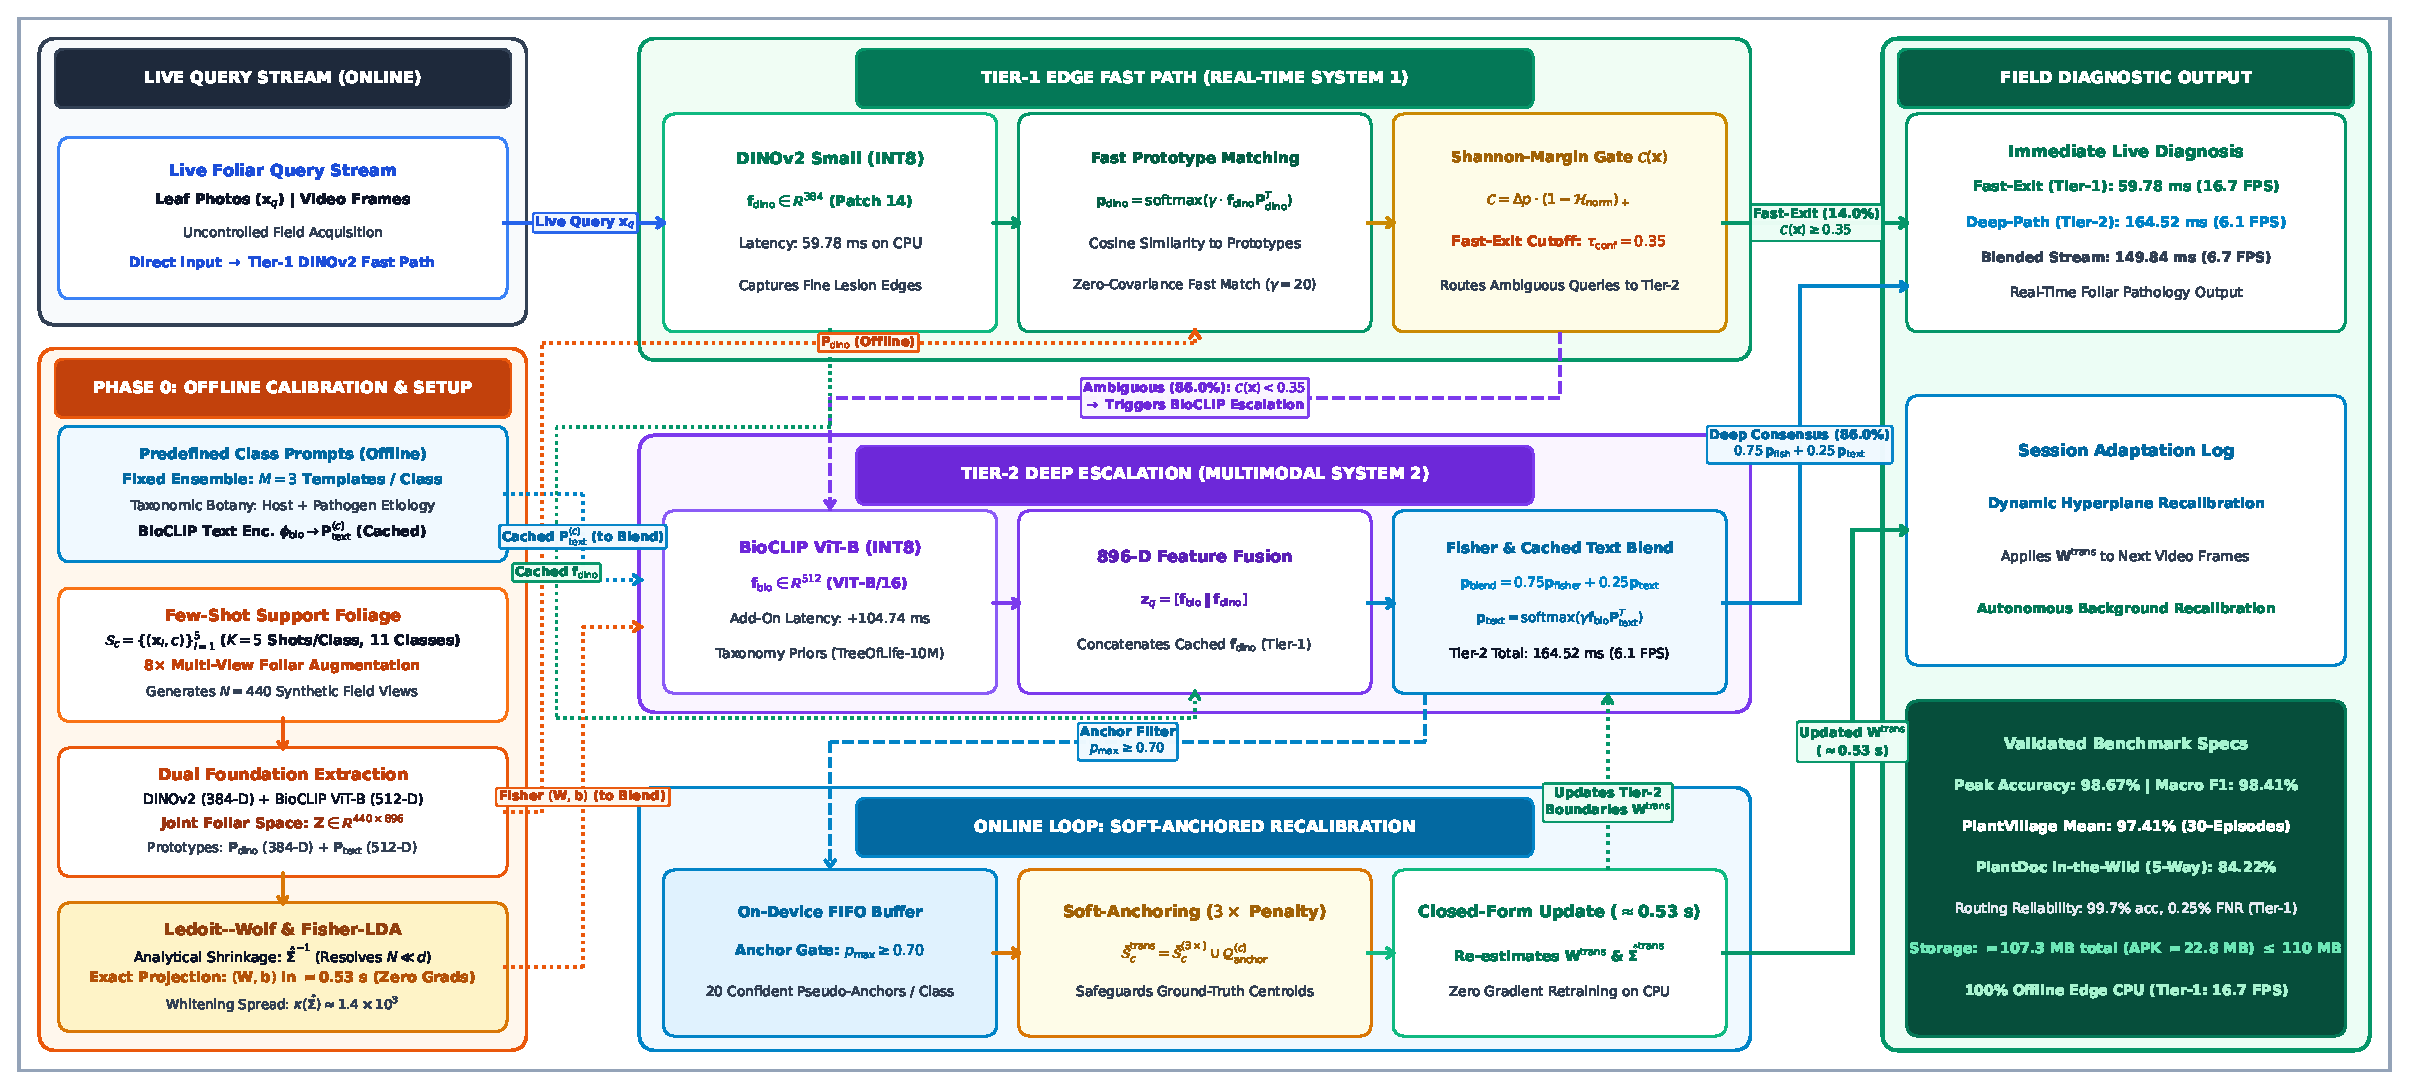
\includegraphics[width=0.88\textwidth]{fig_architecture.pdf}
\caption{Architecture of BioDINO-Edge. Phase~0 (offline) computes Tier-1 visual prototypes and closed-form Fisher-LDA projections while caching botanical text prototypes. During inference, the Shannon-margin uncertainty gate sends routine foliage through Tier-1 fast prototype matching (DINOv2) and escalates ambiguous queries to Tier-2 multimodal consensus (BioCLIP), followed by closed-form soft-anchored transductive recalibration.}
\label{fig:architecture}
\end{figure*}

\subsection{Dual-Foundation Foliar Representation}
\label{sec:feature_extraction}
BioDINO-Edge couples two frozen backbones. DINOv2 provides patch-level features of leaf surface texture and lesion boundaries, while BioCLIP provides organismal taxonomic priors. Concatenating their $\ell_2$-normalized outputs yields an 896-dimensional descriptor that encodes localized symptoms alongside host context.

\subsubsection{Few-Shot Multi-View Support Augmentation}
To mitigate sample covariance rank deficiency and spectral ill-conditioning under scarce reference data ($K = 5$), each support leaf $\mathbf{x} \in \mathcal{S}_c$ is resized to $224 \times 224$ pixels, normalized, and passed through an 8-view stochastic augmentation pipeline approximating field variations. The pipeline applies random horizontal and vertical flips, rotations within $\pm 15^\circ$, and color jitter (brightness, contrast, and saturation factors of $0.2$). Generating eight views per leaf yields $|\tilde{\mathcal{S}}_c| = 8K = 40$ augmented views per class, producing $N = 40C = 440$ total support representations for $C = 11$. This expansion brings the support sample size close to half the joint feature dimension ($d/2 = 448$), which stabilizes the covariance condition number. Although augmented views are not strictly independent, regularized shrinkage prevents numerical degeneracy and guarantees positive-definiteness. For the controlled PlantVillage comparison we use the cached single-view features; Table~\ref{tab:aug_sensitivity} isolates the 8-view expansion. PlantDoc results use the 8-view features throughout.

\subsubsection{Dual-Foundation Embedding Fusion}
Each augmented view $\tilde{\mathbf{x}} \in \tilde{\mathcal{S}}_c$ is passed through the frozen backbones. DINOv2 ViT-S/14 (patch size 14, 384-D)~\cite{oquab2023dinov2} and BioCLIP ViT-B/16~\cite{stevens2024bioclip} extract $\ell_2$-normalized feature vectors:
\begin{equation}
    \mathbf{f}_{\text{dino}} = \frac{\phi_{\text{dino}}(\tilde{\mathbf{x}})}{\|\phi_{\text{dino}}(\tilde{\mathbf{x}})\|_2} \in \mathbb{R}^{384}, \qquad
    \mathbf{f}_{\text{bio}} = \frac{\phi_{\text{bio}}(\tilde{\mathbf{x}})}{\|\phi_{\text{bio}}(\tilde{\mathbf{x}})\|_2} \in \mathbb{R}^{512}.
\end{equation}
Concatenating the two normalized embeddings yields the 896-dimensional joint descriptor:
\begin{equation}
    \mathbf{z} = [\mathbf{f}_{\text{bio}} \,\|\, \mathbf{f}_{\text{dino}}] \in \mathbb{R}^{896}.
\end{equation}
Visual prototypes for the Tier-1 classifier are computed as the normalized mean of the support views:
\begin{equation}
    \mathbf{P}_{\text{dino}}^{(c)} = \text{Normalize}\left(\frac{1}{|\tilde{\mathcal{S}}_c|}\sum_{\tilde{\mathbf{x}} \in \tilde{\mathcal{S}}_c} \mathbf{f}_{\text{dino}}(\tilde{\mathbf{x}})\right),
\end{equation}
yielding the Tier-1 visual prototype matrix $\mathbf{P}_{\text{dino}} \in \mathbb{R}^{C \times 384}$.

\subsubsection{Botanical Taxonomic Prompts and Negation Avoidance}
BioCLIP provides a shared vision--language space, but running text decoders on device costs latency and memory. We therefore define $M = 3$ botanical prompt templates $\{T_c^{(m)}\}_{m=1}^M$ offline for each disease class $c \in \{1, \dots, C\}$. Each template covers three elements:
\begin{enumerate}
    \item \textbf{Host species:} Botanical genus and species (e.g., \textit{Malus domestica}, \textit{Vitis vinifera}, \textit{Solanum tuberosum}).
    \item \textbf{Pathogen name:} Scientific name of the causal agent (e.g., \textit{Venturia inaequalis}, \textit{Guignardia bidwellii}, \textit{Phytophthora infestans}).
    \item \textbf{Visible symptoms:} Diagnostic foliar symptoms (e.g., ``olive-green velvety lesions'', ``tiger-stripe interveinal chlorosis'', ``target-board concentric rings'').
\end{enumerate}
Syntactic negations such as ``healthy leaf without lesions'' or ``no necrotic spots'' are excluded. Vision--language models handle negation poorly~\cite{alhamoud2025vision}, consistent with their bag-of-words, order-insensitive behaviour~\cite{yuksekgonul2023when}: a negated healthy description is encoded close to the disease concepts it mentions rather than away from them. With the BioCLIP text encoder, the three healthy prototypes lie at a mean cosine similarity of 0.557 to the eight disease prototypes when described by negation (range 0.422--0.666), against 0.483 (range 0.359--0.633) for purely positive histological descriptions (``clean vibrant green lamina with smooth intact blade surface''). The same pattern appears end to end: switching the three healthy classes to negated prompts raises transductive FNR from 1.25\% to 2.57\% on the prompt-ablation split. Omitting negations therefore keeps healthy prototypes out of disease clusters and lowers false-negative escape, so every template describes healthy tissue with affirmative terms (e.g., ``clean green foliage'', ``intact smooth leaf lamina'').

During Phase~0, BioCLIP's text encoder $\phi_{\text{bio,txt}}(\cdot)$ encodes each prompt ensemble, and the results are averaged and $\ell_2$-normalized:
\begin{equation}
    \mathbf{P}_{\text{text}}^{(c)} = \text{Normalize}\left(\frac{1}{M}\sum_{m=1}^M \phi_{\text{bio,txt}}(T_c^{(m)})\right) \in \mathbb{R}^{512}.
\end{equation}
The resulting matrix $\mathbf{P}_{\text{text}} \in \mathbb{R}^{C \times 512}$ is cached on device, so there is no runtime tokenization or language-model overhead.

\subsection{Closed-Form Analytical Adaptation via Regularized Fisher-LDA}
\label{sec:fisher_adaptation}

\subsubsection{Multiclass Fisher Linear Discriminant Formulation}
Standard nearest-centroid and cosine-similarity classifiers implicitly assume uniform variance across all feature directions ($\mathbf{\Sigma} = \mathbf{I}$). That assumption does not hold for leaves: shared vegetative structure (such as venation and lamina) creates high-variance directions that mask lesion differences between diseases on the same host. Multiclass Fisher Linear Discriminant Analysis (Fisher-LDA)~\cite{fisher1936use, rao1948utilization} resolves this by weighting features by $\hat{\mathbf{\Sigma}}^{-1}$, which down-weights those shared directions and amplifies low-variance directions containing discriminative lesion symptoms.

Fisher-LDA computes a linear projection matrix $\mathbf{W} \in \mathbb{R}^{C \times d}$ and bias vector $\mathbf{b} \in \mathbb{R}^C$ that maximize between-class scatter $\mathbf{S}_B$ relative to within-class scatter $\mathbf{S}_W$:
\begin{equation}
    \label{eq:fisher_weights}
    \mathbf{W} = [\boldsymbol{\mu}_1, \dots, \boldsymbol{\mu}_C]^T \hat{\mathbf{\Sigma}}^{-1}, \qquad
    b_c = -\frac{1}{2}\boldsymbol{\mu}_c^T \hat{\mathbf{\Sigma}}^{-1}\boldsymbol{\mu}_c - \log C,
\end{equation}
where $\hat{\mathbf{\Sigma}}$ is the regularized pooled within-class covariance matrix ($d = 896$) and class priors are uniform ($\pi_c = 1/C$).

\subsubsection{Analytical Ledoit--Wolf Covariance Shrinkage}
\label{sec:shrinkage}
As established in Section~\ref{sec:covariance_degeneracy}, evaluating Eq.~\eqref{eq:fisher_weights} cannot proceed via direct inversion because the empirical scatter matrix $\mathbf{S}_W$ (Eq.~\eqref{eq:empirical_scatter}) is strictly singular due to rank deficiency ($\text{rank}(\mathbf{S}_W) \le 429 < 896$). To restore invertibility without manual hyperparameter tuning (such as searching over an empirical grid of ridge penalties $\mathbf{S}_W + \epsilon \mathbf{I}$), we apply analytical Ledoit--Wolf shrinkage~\cite{ledoit2004well}, which contracts $\mathbf{S}_W$ toward a spherical target $\nu \mathbf{I}_d$:
\begin{equation}
    \hat{\mathbf{\Sigma}} = (1 - \rho^*)\mathbf{S}_W + \rho^* \nu \mathbf{I}_d, \qquad \nu = \frac{1}{d}\text{Tr}(\mathbf{S}_W).
    \label{eq:lw_target}
\end{equation}
The optimal shrinkage intensity $\rho^* \in (0, 1]$ is determined in closed form by minimizing expected quadratic Frobenius risk:
\begin{equation}
    \rho^* = \min\left(1, \frac{\sum_{i=1}^N \|(\mathbf{z}_i - \boldsymbol{\mu}_{c_i})(\mathbf{z}_i - \boldsymbol{\mu}_{c_i})^T - \mathbf{S}_W\|_F^2}{N^2 \left[\text{Tr}(\mathbf{S}_W^2) - \frac{1}{d}\text{Tr}^2(\mathbf{S}_W)\right]}\right).
    \label{eq:lw_shrinkage}
\end{equation}
This shifts zero eigenvalues to positive values $\tilde{\lambda}_i = (1 - \rho^*)\lambda_i + \rho^* \nu \ge \rho^* \nu > 0$, ensuring that $\hat{\mathbf{\Sigma}}$ is strictly positive-definite and invertible. Its inverse $\hat{\mathbf{\Sigma}}^{-1}$ is solved stably via Cholesky decomposition ($\hat{\mathbf{\Sigma}} = \mathbf{L}\mathbf{L}^T$). Scoring a query $\mathbf{z}$ as $\mathbf{l}_{\text{fisher}} = \mathbf{z}\mathbf{W}^T + \mathbf{b}$ then requires only $C \cdot d$ multiply-accumulate (MAC) operations ($9{,}856$ MACs for $C=11$), requiring minimal on-device computation.

Weighting by $\hat{\mathbf{\Sigma}}^{-1}$ acts as a whitening transform: each eigen-direction with variance $\lambda_i$ is rescaled by $1/\lambda_i$, dampening common leaf morphology while highlighting subtle lesion variations. The condition number
\begin{equation}
    \kappa(\hat{\mathbf{\Sigma}}) = \lambda_{\max}(\hat{\mathbf{\Sigma}}) / \lambda_{\min}(\hat{\mathbf{\Sigma}})
    \label{eq:whitening_spread}
\end{equation}
reflects the dynamic range of this feature rescaling. Because the augmented support views are formed from real leaves, shrinkage guarantees numerical stability across all sample sizes.

\subsection{Adaptive Two-Tier Classification and Edge Deployment}
\label{sec:edge_cascade}

\subsubsection{Tier-1 Fast Path and Shannon Uncertainty Gating}
For an incoming leaf image $\mathbf{x}$, Tier~1 extracts the normalized DINOv2 embedding $\mathbf{f}_{\text{dino}} \in \mathbb{R}^{384}$ and computes fast prototype logits by temperature-scaled cosine similarity against the visual prototypes $\mathbf{P}_{\text{dino}} \in \mathbb{R}^{C \times 384}$:
\begin{equation}
    \label{eq:tier1_logits}
    \mathbf{l}_{\text{dino}} = \gamma \cdot \left(\mathbf{f}_{\text{dino}} \mathbf{P}_{\text{dino}}^T\right), \qquad \gamma = 20.0.
\end{equation}
A softmax yields the fast posterior probabilities:
\begin{equation}
    \label{eq:tier1_softmax}
    \mathbf{p}_{\text{dino}} = \text{softmax}(\mathbf{l}_{\text{dino}}) \in \Delta^{C-1}.
\end{equation}
Tier~1 uses cosine prototype matching only, with no covariance projection, so the Fisher-LDA computation is spent only on queries that need it. The Tier-1 prediction is $\hat{y}_{\text{tier1}} = \arg\max_c p_{\text{dino}, c}$.

Certainty is scored from the same forward pass, so no extra computation is needed. We combine the top-2 margin and normalized entropy into a confidence score $\mathcal{C}(\mathbf{x}) \in [0, 1]$:
\begin{equation}
    \label{eq:shannon_gate}
    \mathcal{C}(\mathbf{x}) = \left(p_{\text{dino}, (1)} - p_{\text{dino}, (2)}\right) \cdot \left(1.0 - \mathcal{H}_{\text{norm}}(\mathbf{x})\right)_+,
\end{equation}
where $p_{\text{dino}, (1)}$ and $p_{\text{dino}, (2)}$ are the top-1 and top-2 posteriors, $(\cdot)_+ = \max(0, \cdot)$, and $\mathcal{H}_{\text{norm}}(\mathbf{x})$ is the normalized Shannon entropy~\cite{shannon1948mathematical}:
\begin{equation}
    \mathcal{H}_{\text{norm}}(\mathbf{x}) = -\frac{1}{\log C}\sum_{c=1}^C p_{\text{dino}, c}\log(p_{\text{dino}, c} + \epsilon),
\end{equation}
with $\epsilon = 10^{-12}$ for numerical stability. The rectifier $(\cdot)_+$ simply guards against floating-point round-off. Ambiguous queries with near-uniform posteriors exhibit high entropy ($\mathcal{H}_{\text{norm}} \to 1$) and negligible margin, driving $\mathcal{C}(\mathbf{x}) \to 0$. When $\mathcal{C}(\mathbf{x}) \ge \tau_{\text{conf}}$ ($\tau_{\text{conf}} = 0.35$, calibrated on validation data), Tier~1 accepts the prediction; otherwise, the query escalates to Tier~2.

\subsubsection{Tier-2 Multimodal Consensus Escalation}
When $\mathcal{C}(\mathbf{x}) < \tau_{\text{conf}}$, the query goes to Tier~2. BioCLIP ViT-B extracts $\mathbf{f}_{\text{bio}} \in \mathbb{R}^{512}$, which is concatenated with the Tier-1 embedding to form $\mathbf{z} = [\mathbf{f}_{\text{bio}} \,\|\, \mathbf{f}_{\text{dino}}] \in \mathbb{R}^{896}$. Two posteriors are then computed: the discriminant visual posterior $\mathbf{p}_{\text{fisher}} = \text{softmax}(\mathbf{z}\mathbf{W}^T + \mathbf{b})$ and the taxonomic text posterior $\mathbf{p}_{\text{text}} = \text{softmax}(\gamma \cdot \mathbf{f}_{\text{bio}}\mathbf{P}_{\text{text}}^T)$. These are fused with Fisher consensus weight $w_{\text{lda}} = 0.75$:
\begin{equation}
    \label{eq:multimodal_blend}
    \mathbf{p}_{\text{blend}} = w_{\text{lda}} \, \mathbf{p}_{\text{fisher}} + (1 - w_{\text{lda}}) \, \mathbf{p}_{\text{text}},
\end{equation}
and the final diagnosis is $\hat{y} = \arg\max_c p_{\text{blend}, c}$. This weighting assigns primary decision confidence ($75\%$) to the sample-adapted visual Fisher geometry, which resolves localized foliar lesion symptoms, while preserving a stabilizing $25\%$ contribution from the botanical language prior to prevent taxonomically implausible misclassifications. Calibrated via grid sweep on validation episodes, $w_{\text{lda}} = 0.75$ achieves the optimal balance between empirical lesion separability and zero-shot semantic regularization.

\subsubsection{Soft-Anchored Transductive Recalibration}
\label{sec:transductive}
In 5-shot calibration, each centroid $\boldsymbol{\mu}_c$ is estimated from only five support leaves. Lighting changes, shadows, and symptom progression can shift prototypes between support images and field queries. To adapt without manual labels, confident Tier-2 queries ($\max_c p_{\text{blend}, c} \ge 0.70$) are buffered into a first-in, first-out (FIFO) queue as reference anchors $\mathcal{Q}_{\text{anchor}}^{(c)}$, limited to 20 anchors per class. Verified support samples receive a $3\times$ weight factor so that pseudo-label drift does not shift class centroids away from confirmed disease definitions:
\begin{equation}
    \label{eq:transductive_set}
    \tilde{\mathcal{S}}_c^{\text{trans}} = \tilde{\mathcal{S}}_c^{(3\times)} \cup \mathcal{Q}_{\text{anchor}}^{(c)}.
\end{equation}
Once the buffer fills during scouting, centroids $\boldsymbol{\mu}_c^{\text{trans}}$ and pooled scatter matrix $\mathbf{S}_W^{\text{trans}}$ are re-estimated, the shrinkage parameter $\rho^*$ is recomputed, and updated projection parameters $(\mathbf{W}^{\text{trans}}, \mathbf{b}^{\text{trans}})$ are resolved via Cholesky substitution. Because query representations are already cached during inference, this update re-executes the identical closed-form algebraic solver as Phase~0 in approximately 0.53\,s, running asynchronously in a background thread so that Tier~1 maintains real-time streaming throughput while subsequent Tier-2 decisions benefit from updated prototypes.

Three design choices keep this update stable and efficient. First, the 0.70 confidence threshold ensures high pseudo-label purity ($\approx$98\%) while avoiding the coverage starvation that collapses accuracy at higher thresholds ($\ge$0.80). Second, the support weight anchors class centroids against manifold drift: the original support leaves are repeated $w_{\mathrm{sup}}$ times so that in the re-estimated centroid
$\boldsymbol{\mu}_c^{\text{trans}} = (w_{\mathrm{sup}}\sum_{\mathbf{x}\in\mathcal{S}_c}\mathbf{x} + \sum_{\mathbf{q}\in\mathcal{Q}_{\text{anchor}}^{(c)}}\mathbf{q}) / (w_{\mathrm{sup}}|\mathcal{S}_c| + |\mathcal{Q}_{\text{anchor}}^{(c)}|)$
the verified leaves outvote pseudo-labels, and $w_{\mathrm{sup}}$ is set per deployment rather than fixed globally. With five support leaves per class and up to twenty anchors, $w_{\mathrm{sup}}=3$ keeps a single support leaf worth roughly one and a half confident anchors on the 11-class benchmark, whereas the field protocol, which draws only two anchors per class, uses $w_{\mathrm{sup}}=1$ or $2$ and no confidence threshold because a fixed threshold there leaves too few eligible anchors. Third, the 20-anchor cap bounds update latency while preventing frequent classes from introducing sample imbalance.

\subsection{Two-Tier Quantized Edge Model Packaging and Android Architecture}
\label{sec:packaging}
Agricultural edge devices operate under limited memory and power budgets, and field connectivity is often unreliable~\cite{sharif2026real,radocaj2025evolution}. BioDINO-Edge therefore never sends a diagnosis over the network: once installed, every query is processed on device without streaming, cloud offloading, or server calls. The framework is partitioned into two INT8-quantized Open Neural Network Exchange (ONNX) binaries, separating a fast standalone engine from an on-demand deep companion.

\textbf{Tier 1 Standalone Engine} (\path{biodino_mobile_int8.onnx}): Packaged inside an APK (occupying $\approx$22.0\,MB on disk). It integrates the DINOv2 Small INT8 backbone, calibrated Phase~0 prototypes, and the Shannon confidence gate executed via the ONNX Runtime C++ execution provider. Installing the APK enables immediate offline diagnosis.

\textbf{Tier 2 Companion Module} (\path{biodino_companion_int8.onnx}): The companion engine occupies $\approx$85.3\,MB on disk, containing the BioCLIP ViT-B INT8 backbone and the 896-dimensional Fisher projection matrix. It is fetched on-demand when high-precision multimodal escalation is requested, functioning completely offline once stored.

Together, both binaries occupy $\approx$107.3\,MB of flash storage on device.

\textbf{On-Device Few-Shot Pathogen Enrollment.} To accommodate field scenarios where agronomists encounter novel or uncataloged foliar pathologies, the Android application integrates an interactive on-device enrollment interface. Users can register a new disease class directly in the field by capturing 1--5 exemplar photos of symptomatic foliage, along with an optional healthy leaf reference from the same host crop. Upon capture, the application extracts foundation embeddings, runs on-device multi-view augmentation, and resolves the regularized discriminant projection via Efficient Java Matrix Library (EJML) Cholesky factorization in sub-second time, enabling immediate subsequent detection entirely offline without network connectivity.

% =============================================================================
% --- END INLINE: 03_methodology.tex ---
% --- BEGIN INLINE: 04_experimental_setup.tex ---
% =============================================================================
% 5. EXPERIMENTAL SETUP
% =============================================================================
\section{Experimental Setup}
\label{sec:experiments_setup}

\subsection{Datasets and Diagnostic Pathology Coverage}
\label{sec:datasets}
We evaluate BioDINO-Edge across two foliar pathology benchmarks with contrasting imaging characteristics:

\subsubsection{PlantVillage Controlled Benchmark}
From the standard PlantVillage benchmark~\cite{mohanty2016plantvillage}, we build a curated 11-class subset of 9{,}385 foliar images from three crops: Apple (\textit{Malus domestica}), Grape (\textit{Vitis vinifera}), and Potato (\textit{Solanum tuberosum}). The classes cover healthy foliage and eight diseases: Apple Scab, Apple Black Rot, Apple Cedar Rust, Grape Black Rot, Grape Esca, Grape Leaf Blight, Potato Early Blight, and Potato Late Blight. This setup evaluates fine-grained lesion identification on the same plant species rather than broad crop separation, providing a genuine test of disease discrimination.

For few-shot calibration, five support images per class ($K=5$) are drawn at random (55 in total), while the remaining 9{,}330 images serve as unseen queries. Backbones are evaluated strictly frozen without fine-tuning on either benchmark, acknowledging potential data overlap within web-scale pre-training corpora.

\subsubsection{PlantDoc In-The-Wild Field Benchmark}
To evaluate diagnostic robustness under challenging field conditions (such as sunlight glare, canopy shadows, soil clutter, and overlapping foliage), we use the in-the-wild PlantDoc benchmark~\cite{singh2020plantdoc}, spanning 27 shared pathology classes across 2{,}668 training images and 252 field test images (\ref{app:plantdoc_official} verifies consistency against the official release). Support and query splits are strictly disjoint ($\mathcal{S} \cap \mathcal{Q} = \emptyset$). We test under two evaluation settings:
\begin{itemize}
    \item \textbf{5-way 5-shot episodic:} Under the standard episodic $N$-way $K$-shot protocol~\cite{snell2017prototypical}, we run 50 independent Monte Carlo episodes. In each episode $e$, 5 classes are drawn without replacement ($\mathcal{C}_e \subset \{1, \dots, 27\}$), and the support set $\mathcal{S}_e$ contains 5 labeled leaves per class (25 total) from the training split. The query set $\mathcal{Q}_e$ contains all test images from those 5 classes (averaging 46.7 query leaves per episode).
    \item \textbf{27-way all-class evaluation:} All 27 classes are evaluated simultaneously (where random-guess accuracy is $1/27 \approx 3.70\%$). The model receives 5 support leaves per class (135 total), expanded by 8-view augmentation to $N = 1{,}080$ feature vectors, and scores all 252 field queries in closed form.
\end{itemize}

\subsection{Evaluation Protocols and Safety Metrics}
\label{sec:metrics}
Experiments on PlantVillage are evaluated over 30 independent Monte Carlo episodes with randomized support splits, reporting mean accuracy $\bar{x}$, standard deviation $\sigma$, 95\% confidence intervals (CI; $95\%\,\text{CI} = \bar{x} \pm 1.96 \cdot \sigma / \sqrt{30}$), and peak single-episode accuracy. Because misclassification costs in precision agriculture are asymmetric, we evaluate safety metrics alongside standard accuracy:
\begin{itemize}
    \item \textbf{Top-1 Accuracy and Macro F1-Score:} The F1-score is macro-averaged across all classes to prevent frequent classes from masking errors on smaller or healthy classes.
    \item \textbf{False-Negative Rate:} The proportion of diseased leaves incorrectly classified as healthy, where false-negative (FN) and true-positive (TP) counts define the rate: $\text{FNR} = \text{FN} / (\text{TP} + \text{FN})$.
    \item \textbf{Cross-Species Confusion Rate:} The proportion of queries misattributed to an entirely different botanical family (e.g., classifying a potato leaf as an apple disease).
    \item \textbf{Area Under the Risk--Coverage Curve (AURC):} For selective classification and confidence gating, we evaluate the trade-off between coverage (fraction of queries processed by the gating rule) and selective risk (error rate among accepted queries). The AURC integrates empirical risk across all coverage levels; lower values denote better uncertainty calibration and safer selective triage.
\end{itemize}

To ensure unbiased cross-domain evaluation, shared parameters ($\gamma = 20.0$, $w_{\text{lda}} = 0.75$, and $\tau_{\text{conf}} = 0.35$) were calibrated strictly on independent PlantVillage validation episodes and applied to PlantDoc without re-tuning. The transductive buffer is adapted to the smaller test volume of PlantDoc (252 total queries across 27 classes): the buffer retains confident predictions capped at two anchors per class, preventing buffer starvation while maintaining high pseudo-label purity. We report both static inductive and transductive results across all benchmarks to separate baseline feature discrimination from dynamic adaptation gains.

\subsection{Edge Hardware Testbed}
\label{sec:edge_hardware_testbed}
On-device profiling is conducted on a physical Samsung Galaxy S24~FE smartphone running Android~17, as detailed in Table~\ref{tab:device_spec}. Neural network inference executes strictly on the ARM64 CPU via ONNX Runtime with per-channel INT8 quantization (4 intra-op threads; GPU and neural accelerators disabled), while closed-form linear algebra runs via EJML. Benchmark latencies and process PSS memory are averaged over 100 iterations following 10 warm-up runs, with thermal stability monitored during continuous operation.

\begin{table}[htbp]
\caption{On-device edge testbed configuration (physical Android device, CPU-only INT8).}
\label{tab:device_spec}
\centering
\footnotesize
\begin{tabular}{ll}
\toprule
\textbf{Hardware / Software Property} & \textbf{System Specification} \\
\midrule
Physical Device & Samsung SM-S721B (Galaxy S24 FE) \\
System-on-Chip (SoC) & Samsung s5e9945 (Exynos 2400e) \\
Operating System & Android 17 (API Level 37) \\
CPU Architecture / Cores & arm64-v8a / 10 Cores \\
Available System RAM & 7,224.3~MB ($\approx$7.2~GB) \\
Inference Engine & ONNX Runtime 1.18.0 (CPUExecutionProvider) \\
Execution Threading & 4 intra-op / 2 inter-op threads \\
Quantization Precision & Static INT8 (NNAPI Disabled) \\
Application Size & Base APK: $\approx$22.8\,MB \\
\bottomrule
\end{tabular}
\end{table}
% --- END INLINE: 04_experimental_setup.tex ---
% --- BEGIN INLINE: 05_results.tex ---
% =============================================================================
% 5. EXPERIMENTAL RESULTS AND PRACTICAL ENGINEERING ANALYSIS
% =============================================================================
\section{Experimental Results and Practical Engineering Analysis}
\label{sec:results}

This section evaluates BioDINO-Edge against operational edge deployment requirements. We first benchmark classification accuracy against few-shot baselines on controlled and in-the-wild datasets (Section~\ref{sec:comparative_results}) and verify statistical significance (Section~\ref{sec:significance}). We then evaluate the contribution of each framework component (Section~\ref{sec:ablation}), measure on-device latency and memory footprints across embedded target hardware (Section~\ref{sec:edge_hardware}), test robustness against sensor noise and parameter variations (Section~\ref{sec:calibration}), and examine per-class diagnostic failure patterns (Section~\ref{sec:per_class}).

% -----------------------------------------------------------------------------
% 5.1 Primary Benchmark Performance and Baseline Evaluation
% -----------------------------------------------------------------------------
\subsection{Primary Benchmark Performance and Baseline Evaluation}
\label{sec:comparative_results}

To benchmark diagnostic accuracy under controlled conditions, Table~\ref{tab:comparative} compares BioDINO-Edge against representative zero-shot and few-shot baseline paradigms. All methods are evaluated across identical support/query partitions, random seeds, and shot counts ($K \in \{1, 5\}$). Extended $K$-shot curves appear in \ref{app:shot_ladder} (Table~\ref{tab:shot_ladder}).

\begin{table*}[htbp]
\caption{Controlled comparison with few-shot baseline paradigms on PlantVillage under identical frozen representations, splits, and seeds (single-view reference features).}
\label{tab:comparative}
\centering

\footnotesize
\setlength{\tabcolsep}{3.5pt}
\begin{tabularx}{\textwidth}{@{}>{\raggedright\arraybackslash}X *{4}{>{\centering\arraybackslash}p{2.6cm}}@{}}
\toprule
& \multicolumn{2}{c}{\textbf{5-way accuracy (\%) ($\uparrow$)}} & \multicolumn{2}{c}{\textbf{11-class, 5-shot (\%) ($\uparrow$)}} \\
\cmidrule(lr){2-3}\cmidrule(lr){4-5}
\textbf{Method} & \textbf{1-shot} & \textbf{5-shot} & \textbf{Accuracy} & \textbf{Macro F1} \\
\midrule
Zero-shot BioCLIP~\cite{stevens2024bioclip} & 38.89$\pm$12.78 & 38.86$\pm$12.79 & 19.18$\pm$0.02 & 18.49 \\
Tip-Adapter~\cite{zhang2022tip} & 45.15$\pm$13.42 & 68.63$\pm$12.80 & 49.97$\pm$1.62 & 46.54 \\
Prototypical Networks~\cite{snell2017prototypical} & 88.44$\pm$9.13 & 97.45$\pm$2.03 & 93.28$\pm$1.24 & 92.47 \\
BioDINO-Edge (inductive, ours) & \underline{88.45$\pm$9.12} & \underline{97.96$\pm$1.85} & \underline{95.08$\pm$1.27} & \underline{94.51} \\
BioDINO-Edge (transductive, ours) & \textbf{93.42$\pm$6.83} & \textbf{98.77$\pm$1.68} & \textbf{97.41$\pm$0.71} & \textbf{97.09} \\
\bottomrule
\end{tabularx}

\vspace{3pt}
\begin{minipage}{\textwidth}
\footnotesize
\textit{Notes.} Bold denotes the best performance in each column; underline denotes second-best. $(\uparrow)$ indicates metrics where higher values are better.
\end{minipage}
\end{table*}

\textbf{Engineering interpretation of baseline performance.} As shown in Table~\ref{tab:comparative}, BioDINO-Edge improves diagnostic accuracy across all few-shot regimes. In the inductive setting, regularized Fisher-LDA projection suppresses common vegetative variance, reaching 95.08\% accuracy. Incorporating transductive anchor recalibration further raises accuracy to 97.41\%, executing entirely on edge CPUs without backpropagation. In contrast, standard unregularized distance metrics underperform because treating all 896 embedding dimensions uniformly leaves predictions vulnerable to dominant leaf veins and glare, while general text prompts in zero-shot adapters lack spatial lesion specificity.

To isolate the impact of our adaptation framework from feature dimensionality and transductive access, Table~\ref{tab:fair_baselines} compares all baselines on identical 896-D features and identical episodes. Following linear-probe evaluations on frozen embeddings~\cite{tian2020rethinking}, we include regularized multinomial logistic regression; we add a closed-form ridge-regression probe in the spirit of differentiable closed-form few-shot solvers~\cite{bertinetto2019r2d2}. Across all inductive comparators on the 896-D features, BioDINO-Edge consistently outperforms Ridge regression, logistic regression, Tip-Adapter, and Prototypical Networks.

Because BioDINO-Edge incorporates transductive recalibration, we also evaluate standard transductive baselines under full-batch query access. In this offline setting with the entire test set visible simultaneously, our re-implementation of LaplacianShot~\cite{ziko2020laplacian} reaches 98.49\% on 11-class PlantVillage (1.08\,pp above BioDINO-Edge), whereas our re-implementations of TIM~\cite{boudiaf2020transductive} and prototype rectification~\cite{liu2020bdcspn} achieve lower accuracy. We also tested whether our regularized Fisher projection could serve as a preprocessing front-end for LaplacianShot. Running Laplacian propagation in the Fisher-projected subspace drops accuracy by 5.7\,pp (from 98.49\% down to 92.84\%). This drop occurs because Fisher-LDA projects the 896 dimensions onto $C-1$ discriminant axes to maximize global class separation, which removes the fine-grained local neighborhood manifold that graph Laplacian smoothing relies on.

\begin{table*}[htbp]
\caption{Comparison with inductive and transductive few-shot baselines on identical 896-D single-view features and episodes (PlantVillage).}
\label{tab:fair_baselines}
\centering

\footnotesize
\setlength{\tabcolsep}{4pt}
\begin{tabularx}{\textwidth}{@{}>{\raggedright\arraybackslash}X *{4}{>{\centering\arraybackslash}p{2.3cm}}@{}}
\toprule
\textbf{Method (features)} & \textbf{5-way 1-shot} & \textbf{5-way 5-shot} & \textbf{11-class, 5-shot} & \textbf{11-class F1} \\
\midrule
\multicolumn{5}{@{}l}{\textit{Inductive: training-free and closed-form linear probes}}\\
Tip-Adapter (512-D BioCLIP, as published) & 45.15$\pm$13.42 & 68.63$\pm$12.80 & 49.97$\pm$1.62 & 46.54 \\
Tip-Adapter (896-D, ours) & -- & 73.02$\pm$12.21 & 55.60$\pm$1.67 & 51.15 \\
Ridge classifier (896-D) & -- & 97.74$\pm$1.82 & 93.83$\pm$1.08 & 92.47 \\
Multinomial logistic (896-D) & -- & 97.67$\pm$1.82 & 93.63$\pm$1.02 & 92.52 \\
Prototypical Networks (896-D) & 88.44$\pm$9.13 & 97.45$\pm$2.03 & 93.28$\pm$1.24 & 92.47 \\
BioDINO-Edge inductive (896-D) & \underline{88.45$\pm$9.12} & 97.96$\pm$1.85 & 95.08$\pm$1.27 & 94.51 \\
\midrule
\multicolumn{5}{@{}l}{\textit{Transductive: same features, same episodes}}\\
Prototype rectification~\cite{liu2020bdcspn} (896-D) & -- & 98.22$\pm$1.58 & 94.82$\pm$0.59 & 93.66 \\
TIM~\cite{boudiaf2020transductive} (896-D) & -- & 96.43$\pm$2.47 & 91.40$\pm$1.38 & 89.20 \\
LaplacianShot~\cite{ziko2020laplacian} (896-D) & -- & \textbf{99.50$\pm$0.82} & \textbf{98.49$\pm$0.59} & \textbf{98.70} \\
BioDINO-Edge transductive (896-D) & \textbf{93.42$\pm$6.83} & \underline{98.77$\pm$1.68} & \underline{97.41$\pm$0.71} & \underline{97.09} \\
\bottomrule
\end{tabularx}

\vspace{3pt}
\begin{minipage}{\textwidth}
\footnotesize
\textit{Notes.} Evaluated across 30 episodes for 11-class and 50 episodes for 5-way tasks on identical support and query splits. Upper block: inductive methods; lower block: transductive methods. All rows are our re-implementations on these shared features and episodes. Bold marks the best performance per column; underline denotes second-best. Baseline hyperparameters are detailed in \ref{app:repro}.
\end{minipage}
\end{table*}

\textbf{Practical edge deployment: streaming queries and unconstrained field conditions.} While LaplacianShot achieves strong accuracy on fixed offline query pools, its formulation requires constructing a pairwise nearest-neighbor graph over the entire query batch simultaneously. In real-world edge deployment, scouting occurs sequentially rather than in offline pools. As evaluated in Table~\ref{tab:batchsize}, when queries arrive one leaf at a time without batch buffering, LaplacianShot's accuracy drops to 93.12\%, whereas BioDINO-Edge maintains a constant 96.12\% accuracy because its fixed-capacity anchor queue operates independently of external batch buffering sizes.

\begin{table}[htbp]
\caption{Diagnostic accuracy under sequential and buffered query streaming (11-class, 5-shot on PlantVillage; single-view reference).}
\label{tab:batchsize}
\centering

\footnotesize
\setlength{\tabcolsep}{4pt}
\begin{tabular*}{\columnwidth}{@{\extracolsep{\fill}}lccc}
\toprule
\textbf{Strategy} & \textbf{LaplacianShot (\%)} & \textbf{BioDINO-Edge (\%)} & \textbf{$\Delta$ (pp)} \\
\midrule
One leaf at a time (no buffer) & 93.12 & \textbf{96.12} & $+3.00$ \\
Growing buffer, 25 & 86.50 & \textbf{96.12} & $+9.62$ \\
Growing buffer, 100 & 90.17 & \textbf{96.12} & $+5.96$ \\
Growing buffer, 200 & 93.48 & \textbf{96.12} & $+2.65$ \\
Whole query set (lab protocol) & \textbf{96.38} & 96.12 & $-0.25$ \\
\bottomrule
\end{tabular*}

\vspace{3pt}
\begin{minipage}{\columnwidth}
\footnotesize
\textit{Notes.} Evaluated across 8 paired episodes with 600 queries each. Positive $\Delta$ indicates a gain for BioDINO-Edge ($p < 0.01$ for streaming and buffered rows; $p = 0.68$ for full-batch query access).
\end{minipage}
\end{table}

Table~\ref{tab:plantdoc_context} extends this evaluation to unconstrained field imagery via the PlantDoc benchmark~\cite{singh2020plantdoc}. In 5-way 5-shot episodic testing over 50 Monte Carlo episodes, BioDINO-Edge reaches 84.94\% accuracy. In the simultaneous 27-class stress test over 252 field test leaves, it achieves 52.38\% accuracy and 52.52\% macro F1.

\begin{table}[htbp]
\caption{In-the-wild field evaluation of BioDINO-Edge on PlantDoc.}
\label{tab:plantdoc_context}
\centering
\footnotesize
\setlength{\tabcolsep}{4pt}
\begin{tabularx}{\columnwidth}{@{}>{\raggedright\arraybackslash}Xcccc@{}}
\toprule
\textbf{Evaluation Regime} & \textbf{Classes} & \textbf{Shots} & \textbf{Inductive (\%) ($\uparrow$)} & \textbf{Transductive (\%) ($\uparrow$)} \\
\midrule
5-way 5-shot episodic (PlantDoc train/test splits) & 5 & 5 & \underline{82.60$\pm$11.49} & \textbf{84.94$\pm$11.15} \\
All-class stress test (simultaneous) & 27 & 5 & \underline{48.81} & \textbf{52.38} \\
\bottomrule
\end{tabularx}

\vspace{3pt}
\begin{minipage}{\columnwidth}
\footnotesize
\textit{Notes.} 5-way values report mean $\pm$ std across 50 Monte Carlo episodes. Bold marks top performance; underline denotes second-best.
\end{minipage}
\end{table}

\ref{app:plantdoc_official} confirms that headline results on the official PlantDoc release show no statistically significant difference (27-way $p=0.33$; 5-way $p=0.25$), demonstrating robustness across dataset redistributions. PlantDoc presents severe environmental challenges: uneven lighting, overlapping foliage, and complex background clutter. Prior cross-dataset evaluations, such as the study by Zhao et al.~\cite{zhao2026lightweight}, report 44.81\% under direct unadapted transfer and 54.24\% following unsupervised target calibration. In the few-shot setting, BioDINO-Edge achieves 52.38\% accuracy across all 27 field classes by adapting directly to labeled support in closed form without iterative retraining. Combining cached botanical text prototypes with analytical Fisher projections provides a stable diagnostic anchor in challenging in-the-wild scenes.

Table~\ref{tab:plantdoc_laplacian} reports the corresponding transductive comparison against LaplacianShot on PlantDoc: BioDINO-Edge outperforms LaplacianShot by $+21.82$\,pp on the 27-way stress test (52.38\% vs.\ 30.56\%) and $+19.21$\,pp at 5-way 5-shot (84.94\% vs.\ 65.73\%). In cluttered field scenes, nearest-neighbor graph propagation breaks down under visual domain shift, whereas BioDINO-Edge maintains high accuracy through regularized covariance projection.

\begin{table}[htbp]
\caption{Transductive comparison against LaplacianShot on PlantDoc (identical 8-view support features).}
\label{tab:plantdoc_laplacian}
\centering

\footnotesize
\setlength{\tabcolsep}{4pt}
\begin{tabular*}{\columnwidth}{@{\extracolsep{\fill}}lccc}
\toprule
\textbf{Regime} & \textbf{LaplacianShot (\%)} & \textbf{BioDINO-Edge (\%)} & \textbf{$\Delta$ (pp)} \\
\midrule
27-way, 252 field queries & 30.56 & \textbf{52.38} & $+21.82$ \\
5-way 5-shot, 50 episodes & 65.73 & \textbf{84.94} & $+19.21$ \\
\bottomrule
\end{tabular*}

\vspace{3pt}
\begin{minipage}{\columnwidth}
\footnotesize
\textit{Notes.} 5-way values report mean accuracy across 50 paired episodes ($p = 1.15 \times 10^{-12}$; 46 wins, 3 losses, 1 tie). Bold denotes best performance.
\end{minipage}
\end{table}

% -----------------------------------------------------------------------------
% 5.2 Statistical Significance and Hypothesis Testing
% -----------------------------------------------------------------------------
\subsection{Statistical Significance and Hypothesis Testing}
\label{sec:significance}
\label{sec:transductive_validation}

To assess the statistical significance of transductive recalibration over the inductive baseline, Table~\ref{tab:paired_test} reports paired hypothesis testing across 30 independent Monte Carlo episodes on PlantVillage.

\begin{table}[htbp]
\caption{Paired statistical evaluation of inductive vs.\ transductive inference over 30 identical episodes (PlantVillage, 5-shot; single-view reference).}
\label{tab:paired_test}
\centering

\footnotesize
\setlength{\tabcolsep}{3pt}
\begin{tabular*}{\columnwidth}{@{\extracolsep{\fill}}lcccc}
\toprule
\textbf{Inference Mode} & \textbf{Accuracy (\%)} & \textbf{Paired $\Delta$ (pp)} & \textbf{Win/Loss} & \textbf{$p$-value} \\
\midrule
Inductive (baseline) & 95.08 $\pm$ 1.27 & -- & -- & -- \\
Transductive (recalibrated) & \textbf{97.41 $\pm$ 0.71} & \textbf{+2.33} $[1.91, 2.74]$ & \textbf{30 / 0} & $2.2\times 10^{-12}$ \\
\bottomrule
\end{tabular*}

\vspace{3pt}
\begin{minipage}{\columnwidth}
\footnotesize
\textit{Notes.} Evaluated across 30 identical Monte Carlo support/query splits. Two-tailed paired $t$-test ($t(29)=11.57, p=2.2\times 10^{-12}$); Wilcoxon signed-rank test ($W=0.0, p=1.9\times 10^{-9}$). Effect size Cohen's $d_z = 2.11$ indicates a substantial practical gain.
\end{minipage}
\end{table}

\textbf{Statistical interpretation.} Table~\ref{tab:paired_test} confirms that transductive recalibration yields a statistically significant improvement over inductive classification ($+2.33$\,pp mean gain, $p < 10^{-11}$). Transductive recalibration outperforms the inductive model across all 30 evaluated episodes (a 30-win, 0-loss record), exhibiting a large standardized effect size (Cohen's $d_z = 2.11$). These results verify that closed-form pseudo-label recalibration reliably corrects prototype drift across randomized support selections.

% -----------------------------------------------------------------------------
% 5.3 Systematic Component Ablation
% -----------------------------------------------------------------------------
\subsection{Systematic Component Ablation}
\label{sec:ablation}

To isolate the contribution of each architectural module, Table~\ref{tab:ablation} presents a step-by-step ablation on the canonical 11-class PlantVillage benchmark under identical 5-shot splits.

\begin{table}[htbp]
\caption{Systematic ablation of BioDINO-Edge architectural components on PlantVillage.}
\label{tab:ablation}
\centering

\footnotesize
\setlength{\tabcolsep}{3pt}
\begin{tabular*}{\columnwidth}{@{\extracolsep{\fill}}lcc}
\toprule
\textbf{Configuration / Component} & \textbf{Acc. (\%) ($\uparrow$)} & \textbf{Macro F1 (\%) ($\uparrow$)} \\
\midrule
(1) Fast-Path DINOv2 Small alone & 87.26 & 85.36 \\
(2) Deep-Path BioCLIP ViT-B alone & 92.60 & 89.88 \\
(3) Text Prototypes Only & 19.20 & 18.55 \\
(4) Static Cosine Blend (raw 5-shot) & 94.16 & 92.55 \\
(5) Static Cosine Blend (8-view aug.) & 93.90 & 91.58 \\
(6) + Regularized Fisher Alignment & \underline{96.05} & \underline{94.83} \\
(7) + Transductive Recalibration (Single Run) & \textbf{98.06} & \textbf{97.45} \\
\midrule
Full System (Peak Statistical Episode) & \textbf{98.67} & \textbf{98.41} \\
\bottomrule
\end{tabular*}

\vspace{3pt}
\begin{minipage}{\columnwidth}
\footnotesize
\textit{Notes.} Evaluated on 11-class PlantVillage (5-shot, 9,330 queries) using single-view reference features, except row (5), which isolates 8-view augmentation. Bold marks top performance; underline denotes second-best.
\end{minipage}
\end{table}

\textbf{Component analysis:}
\begin{enumerate}
    \item \textbf{Dual-Backbone Synergy:} DINOv2 alone reaches 87.26\% (capturing fine lesion boundaries for fast-path inference), while BioCLIP alone achieves 92.60\% (providing global taxonomic context). Combining both encoders into an 896-D representation outperforms either standalone model.
    \item \textbf{Regularized Fisher Alignment (+1.89\,pp Gain):} Replacing isotropic cosine matching (94.16\%) with regularized Fisher-LDA increases accuracy to 96.05\%, effectively attenuating dominant vegetative variance.
    \item \textbf{Transductive Recalibration (+2.01\,pp Gain):} Updating prototypes and covariance estimates using high-confidence query anchors raises accuracy from 96.05\% to 98.06\% (peaking at 98.67\%), correcting prototype drift from sparse initial support leaves.
\end{enumerate}

Table~\ref{tab:feature_ablation} evaluates the individual contribution of each foundation encoder across 30 identical episodes. Removing DINOv2 drops transductive accuracy by 0.90\,pp (from 97.41\% to 96.51\%), while removing BioCLIP drops it by 1.87\,pp (to 95.54\%). This confirms that localized spatial representations and global taxonomic priors provide complementary diagnostic signals.

\begin{table}[htbp]
\caption{Contribution of each foundation encoder to Fisher-LDA classification (30 identical 5-shot episodes, mean $\pm$ std; single-view reference).}
\label{tab:feature_ablation}
\centering

\footnotesize
\setlength{\tabcolsep}{4pt}
\begin{tabular*}{\columnwidth}{@{\extracolsep{\fill}}lccc}
\toprule
\textbf{Fisher Feature Space} & \textbf{Dim} & \textbf{Inductive (\%) ($\uparrow$)} & \textbf{Transductive (\%) ($\uparrow$)} \\
\midrule
BioCLIP + DINOv2 (Full) & 896 & \textbf{95.08$\pm$1.27} & \textbf{97.41$\pm$0.71} \\
BioCLIP alone & 512 & \underline{94.31$\pm$1.25} & \underline{96.51$\pm$0.90} \\
DINOv2 alone & 384 & 90.60$\pm$2.02 & 95.54$\pm$1.03 \\
\bottomrule
\end{tabular*}
\end{table}

\textbf{Component evaluation under unconstrained field conditions.} While Table~\ref{tab:ablation} evaluates components on clean laboratory leaves, Table~\ref{tab:plantdoc_ablation} tests the identical component ladder on unconstrained field imagery across 27 crop classes in PlantDoc.

On unconstrained field imagery spanning 27 disparate crop classes, the static multi-backbone blend achieves 54.37\% accuracy, benefiting from the robust zero-shot taxonomic grounding of BioCLIP paired with DINOv2. Fitting a pooled within-class covariance across 27 diverse plant species with varied outdoor lighting and soil backgrounds introduces variance into the empirical scatter estimate, resulting in 48.81\% for inductive Fisher-LDA. Transductive anchor recalibration recovers accuracy to 52.38\% (and 52.52\% macro F1) by dynamically refining prototypes and covariance with high-confidence field queries. This demonstrates how test-time adaptation effectively counteracts domain shift when deploying to unstructured agricultural environments.

\begin{table}[htbp]
\caption{PlantDoc component ladder (27-way, 5-shot, single run over 252 field queries; 8-view support expansion).}
\label{tab:plantdoc_ablation}
\centering

\footnotesize
\setlength{\tabcolsep}{3pt}
\begin{tabular*}{\columnwidth}{@{\extracolsep{\fill}}lcc}
\toprule
\textbf{Configuration / Component} & \textbf{Acc. (\%) ($\uparrow$)} & \textbf{Macro F1 (\%) ($\uparrow$)} \\
\midrule
(1) Text prototypes only & 34.92 & 29.34 \\
(2) Fast-path DINOv2 Small alone & 38.89 & 35.32 \\
(3) Deep-path BioCLIP ViT-B alone & 48.81 & 50.11 \\
(4) Static logit blend ($0.65$ bio $+$ $0.35$ dino) & \textbf{54.37} & \textbf{54.88} \\
(5) $+$ Regularized Fisher alignment (inductive) & 48.81 & 47.51 \\
(6) $+$ Transductive recalibration & \underline{52.38} & \underline{52.52} \\
\bottomrule
\end{tabular*}

\vspace{3pt}
\begin{minipage}{\columnwidth}
\footnotesize
\textit{Notes.} Evaluated on 27 field classes (135 support leaves, 252 test queries; 8-view support expansion). Bold denotes top performance; underline denotes second-best.
\end{minipage}
\end{table}

\textbf{Quantization resilience: FP32 vs.\ INT8.} To verify numerical stability on edge runtimes, Table~\ref{tab:quantization} compares the pipeline executed in 32-bit floating-point (FP32) against 8-bit integer (INT8) quantized ONNX binaries on identical splits. Quantizing the foundation backbones delivers an approximate $4\times$ reduction in model storage footprint (from $\approx$430\,MB down to 107.3\,MB total on-device storage) while reducing runtime memory bandwidth. While individual intermediate feature stages exhibit minor sensitivity to integer rounding (up to 1.99\,pp on PlantDoc), the closed-form regularized projection and transductive recalibration effectively buffer this precision loss. End-to-end transductive accuracy degrades by only 0.24\,pp on PlantVillage (98.32\% to 98.08\%) and 0.40\,pp on PlantDoc (51.19\% to 50.79\%); because this quantization audit executes in a standalone ONNX runtime harness on an independent support sample, its absolute baseline numbers differ slightly from the headline evaluations in Tables~\ref{tab:plantdoc_context} and~\ref{tab:plantdoc_ablation}, while isolating the relative FP32 vs.\ INT8 delta. These results confirm that BioDINO-Edge preserves diagnostic precision under 8-bit quantization.

\begin{table}[htbp]
\caption{Full-pipeline diagnostic accuracy under FP32 versus INT8 ONNX execution.}
\label{tab:quantization}
\centering

\footnotesize
\setlength{\tabcolsep}{4pt}
\begin{tabular*}{\columnwidth}{@{\extracolsep{\fill}}llccc}
\toprule
\textbf{Dataset} & \textbf{Stage} & \textbf{FP32 (\%) ($\uparrow$)} & \textbf{INT8 (\%) ($\uparrow$)} & \textbf{$\Delta$ (pp)} \\
\midrule
PlantVillage (11) & Tier-1 DINOv2 & 87.33 & 87.59 & $+0.26$ \\
 & BioCLIP alone & 92.71 & 92.29 & $-0.42$ \\
 & Fisher ensemble & 96.29 & 96.68 & $+0.39$ \\
 & $+$ transductive & 98.32 & 98.08 & $-0.24$ \\
\midrule
PlantDoc (27) & Tier-1 DINOv2 & 40.87 & 40.08 & $-0.79$ \\
 & BioCLIP alone & 51.59 & 50.00 & $-1.59$ \\
 & Fisher ensemble & 49.21 & 47.22 & $-1.99$ \\
 & $+$ transductive & 51.19 & 50.79 & $-0.40$ \\
\bottomrule
\end{tabular*}

\vspace{3pt}
\begin{minipage}{\columnwidth}
\footnotesize
\textit{Notes.} Single-split audit using 8-view support expansion across identical splits. $\Delta$ denotes INT8 relative to FP32.
\end{minipage}
\end{table}

% -----------------------------------------------------------------------------
% 5.4 Computational Cost and Real-Time Edge Feasibility
% -----------------------------------------------------------------------------
\subsection{Computational Cost and Real-Time Edge Feasibility}
\label{sec:edge_hardware}

To demonstrate practical utility for field agronomists and autonomous scouting platforms, we evaluate the standalone BioDINO-Edge Android application on the commodity handset detailed in Table~\ref{tab:device_spec}. Execution runs entirely on-device using CPU threads via INT8 ONNX Runtime, ensuring dependable offline diagnostics in remote agricultural environments without cloud access or dedicated AI accelerators.

\textbf{On-device latency profiling.} Table~\ref{tab:device_perf} quantifies the on-device diagnostic latency across individual pipeline stages on the physical mobile CPU. Tier-1 fast-path execution requires 59.78\,ms, while an escalated Tier-2 query takes 164.52\,ms. On the 11-image physical handset test set, cascaded pipeline latency averages 145.37\,ms with an 18.00\% fast-exit acceptance ratio (Table~\ref{tab:hardware_footprint}). Across the full 30-episode stream (9,330 queries), factoring in the 14.02\% multi-episode fast-exit rate yields an average streaming latency of 149.84\,ms ($\approx$6.7\,FPS; Table~\ref{tab:tier_routing}), safely satisfying the 170\,ms real-time design budget with a 95th-percentile tail latency of 196.36\,ms.

\begin{table}[htbp]
\caption{Measured on-device diagnostic latency breakdown on Samsung Galaxy S24 FE.}
\label{tab:device_perf}
\centering

\footnotesize
\begin{tabularx}{\textwidth}{@{}>{\raggedright\arraybackslash}X *{3}{>{\centering\arraybackslash}p{2.8cm}}@{}}
\toprule
\textbf{Pipeline Stage / Component} & \textbf{Mean$\pm$std (ms) ($\downarrow$)} & \textbf{Median (ms) ($\downarrow$)} & \textbf{$p_{95}$ Latency (ms) ($\downarrow$)} \\
\midrule
Input preprocessing \& normalization & 2.59$\pm$0.67 & 2.36 & 4.36 \\
Tier-1 DINOv2 Small visual encoder & 57.18$\pm$9.13 & 51.50 & 68.84 \\
Uncertainty gate routing decision & $<$0.01 & $<$0.01 & $<$0.01 \\
Tier-2 BioCLIP ViT-B encoder \& Fisher solve & 104.74$\pm$17.39 & 94.20 & 124.97 \\
Classification output assembly & $<$0.01 & $<$0.01 & $<$0.01 \\
\midrule
\textbf{Cascaded pipeline end-to-end (ours)} & \textbf{145.37$\pm$47.61} & \textbf{147.77} & \textbf{196.36} \\
Monolithic Tier-2 executed on all queries & 164.52$\pm$26.77 & 148.73 & 196.36 \\
\bottomrule
\end{tabularx}

\vspace{3pt}
\begin{minipage}{\textwidth}
\footnotesize
\textit{Notes.} Evaluated over 100 test iterations on physical mobile CPU cores under INT8 precision. Here, $p_{95}$ denotes the 95th-percentile tail latency.
\end{minipage}
\end{table}

\textbf{Hardware resource footprint and throughput.} Table~\ref{tab:hardware_footprint} details on-device resource usage and stability. Peak physical memory is 497.45\,MB PSS, meeting the 500\,MB operating budget ($M_{\max}$) and enabling execution on devices with as little as 2--4\,GB of available RAM. Under continuous operation for 10 minutes, throughput settles to 4.26\,FPS under thermal load, maintaining interactive responsiveness for shutter-triggered field scouting.

\begin{table}[htbp]
\caption{Hardware resource utilization, memory footprint, and operational throughput on Samsung Galaxy S24 FE.}
\label{tab:hardware_footprint}
\centering

\footnotesize
\setlength{\tabcolsep}{4pt}
\begin{tabular*}{\textwidth}{@{\extracolsep{\fill}}lc}
\toprule
\textbf{Hardware Resource / Deployment Metric} & \textbf{Measured Value} \\
\midrule
Peak physical memory footprint (PSS RAM) & \textbf{497.45 MB} \\
Tier-1 cold model initialization & 323.92 ms \\
Tier-2 companion model initialization & 447.71 ms \\
Standalone application package (Base APK size) & $\approx$22.8 MB \\
Fast-exit acceptance ratio (on-device test set) & 18.00\% \\
Interactive burst throughput (Tier-1 fast path) & $\approx$16.7 FPS (59.78 ms) \\
Sustained continuous throughput under thermal load & \textbf{4.26 FPS} (600\,s continuous stress) \\
Android thermal status during 600\,s soak & 2 $\rightarrow$ 3 (light $\rightarrow$ moderate) \\
\bottomrule
\end{tabular*}

\vspace{3pt}
\begin{minipage}{\textwidth}
\footnotesize
\textit{Notes.} Physical measurements recorded on ARM64 CPU with background OS processes active. Memory tracks total PSS.
\end{minipage}
\end{table}

\textbf{On-device closed-form adaptation.} Table~\ref{tab:adaptation_breakdown} breaks down the on-device computational cost of adapting BioDINO-Edge to novel foliar pathologies on the mobile CPU. Initializing a complete 11-class diagnostic catalog (5 support leaves per class expanded to 440 views) requires a one-time feature extraction pass of 88.06\,s ($\approx$200.1\,ms per augmented view, or $\approx$1.6\,s per leaf). For in-field enrollment of an individual novel disease class (5 leaves, 40 views), feature extraction requires only $\approx$8.0\,s. Following feature extraction, regularized covariance estimation and discriminant parameter solving are strictly closed-form, executing in just 533.99\,ms of algebraic computation on the mobile CPU.

\begin{table}[htbp]
\caption{Closed-form adaptation computational cost breakdown on edge CPU ($N=440$, $d=896$, $C=11$).}
\label{tab:adaptation_breakdown}
\centering

\footnotesize
\begin{tabularx}{\textwidth}{@{}>{\raggedright\arraybackslash}X *{2}{>{\centering\arraybackslash}p{4.2cm}}@{}}
\toprule
\textbf{Adaptation Pipeline Stage} & \textbf{Execution Time (ms) ($\downarrow$)} & \textbf{Algorithmic Complexity} \\
\midrule
Support feature extraction (440 augmented views) & 88,055.60 & $O(N(C_{\text{dino}}+C_{\text{bio}}))$ \\
Empirical scatter matrix accumulation & 146.19$\pm$2.15 & $O(Nd^2)$ \\
Frobenius Ledoit--Wolf shrinkage parameter estimation & 4.49$\pm$0.85 & $O(Nd)$ \\
Cholesky decomposition of regularized covariance & 332.00$\pm$2.52 & $O(d^3/3)$ \\
Discriminant projection solve ($W, b$) & 51.31$\pm$3.68 & $O(Cd^2)$ \\
\midrule
\textbf{Algebraic adaptation total (Closed-Form)} & \textbf{533.99$\pm$6.29} & $O(d^3/3 + Nd^2)$ \\
Complete end-to-end adaptation (Extraction + Algebra) & 88,589.60 & $O(N(C_{\text{dino}}+C_{\text{bio}}) + d^3/3)$ \\
\bottomrule
\end{tabularx}
\end{table}

\FloatBarrier
% -----------------------------------------------------------------------------
% 5.5 Robustness, Environmental Noise, and Sensitivity Analysis
% -----------------------------------------------------------------------------
\subsection{Robustness and Sensitivity Analysis}
\label{sec:calibration}
\label{sec:aug_sensitivity}

This section evaluates the operational robustness and sensitivity of BioDINO-Edge across three core practical dimensions: (i) confidence calibration, threshold selection, and selective routing trade-offs (Figs.~\ref{fig:risk_coverage}--\ref{fig:tau_sensitivity}, Tables~\ref{tab:threshold_sweep}--\ref{tab:tier_routing}); (ii) hyperparameter stability during continuous field streaming (Table~\ref{tab:transductive_sensitivity}); and (iii) the impact of multi-view support generation on Ledoit--Wolf shrinkage and covariance conditioning (Table~\ref{tab:aug_sensitivity}).

\textbf{Confidence calibration and selective routing dynamics.} Fig.~\ref{fig:risk_coverage} evaluates confidence estimation quality using the AURC metric. The dual-metric Shannon gate score achieves an AURC of 3.33\%, outperforming raw maximum softmax probability (3.95\%) and approaching full Tier-2 refined consensus (1.75\%).

Fig.~\ref{fig:tau_sensitivity} evaluates how routing performance responds to continuous threshold variations across $\tau \in [0.05, 0.70]$. As $\tau$ increases, the fast-exit rate declines monotonically from over 60\% to under 5\%, while Tier-1 accepted accuracy rises from 94.0\% and stays above 99.5\% for $\tau \ge 0.35$. Sweeps across split episode subsets (episodes 0--14 for tuning vs.\ 15--29 for testing) yield identical saturation thresholds, indicating that $\tau = 0.35$ generalizes reliably across independent support sets.

\begin{figure}[!htbp]
\centering
\begin{minipage}[b]{0.48\textwidth}
  \centering
  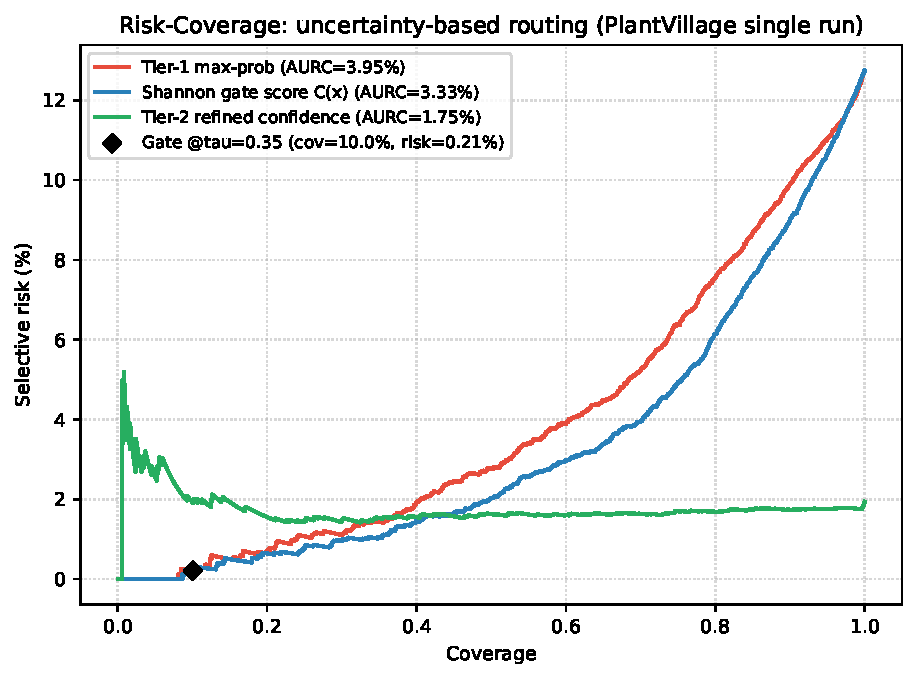
\includegraphics[width=0.96\linewidth]{fig_risk_coverage.pdf}
  \caption{Risk--coverage curves comparing raw Tier-1 maximum softmax probability, the dual-metric Shannon gate score $\mathcal{C}(\mathbf{x})$, and Tier-2 refined consensus confidence (canonical single run). The black diamond marks the deployed operating point at $\tau=0.35$ (10.0\% coverage at 0.21\% selective risk on this episode).}
  \label{fig:risk_coverage}
\end{minipage}\hfill
\begin{minipage}[b]{0.48\textwidth}
  \centering
  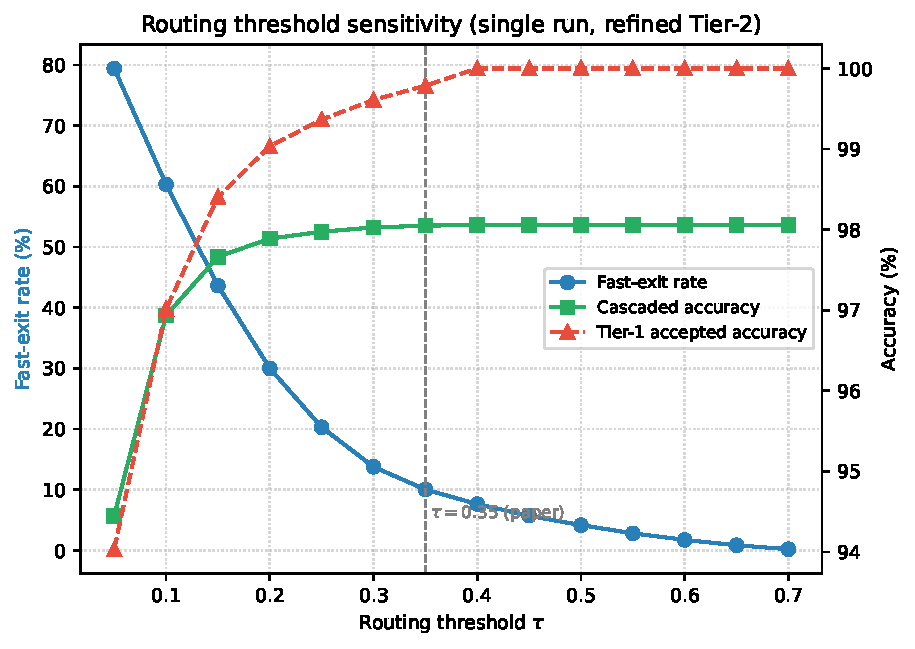
\includegraphics[width=0.96\linewidth]{fig_tau_sensitivity.pdf}
  \caption{Parametric routing-threshold sensitivity sweep across $\tau \in [0.05, 0.70]$ under refined Tier-2 inference. Blue circles (left axis) display fast-exit coverage (\%); green squares and red triangles (right axis) display full cascaded and Tier-1 accepted accuracies (\%). The vertical dashed line marks the deployed operating point ($\tau=0.35$).}
  \label{fig:tau_sensitivity}
\end{minipage}
\end{figure}

Table~\ref{tab:threshold_sweep} compares discrete routing policies across $\tau$. Aggressive policies ($\tau \le 0.20$) maximize fast-exit throughput (up to 61.76\% coverage and 99.83\,ms latency) but reduce Tier-1 accuracy below 99\%, allowing diseased leaves to escape undetected. Conservative policies ($\tau \ge 0.50$) ensure 100\% Tier-1 accuracy but restrict fast-exit coverage to only 5.15\%, diminishing latency benefits. Setting $\tau = 0.35$ balances these constraints, achieving 99.69\% Tier-1 accuracy with a 14.02\% fast-exit rate.

\begin{table}[htbp]
\caption{Selective routing policy sensitivity across gating threshold ($\tau$) sweeps.}
\label{tab:threshold_sweep}
\centering

\footnotesize
\setlength{\tabcolsep}{5pt}
\begin{tabularx}{\textwidth}{@{}>{\raggedright\arraybackslash}X *{4}{>{\centering\arraybackslash}p{2.3cm}}@{}}
\toprule
\textbf{Threshold Policy} & \textbf{Fast-Exit (\%)} & \textbf{Tier-1 Acc. (\%)} & \textbf{Cascaded Acc. (\%)} & \textbf{Latency (ms)} \\
\midrule
Aggressive ($\tau=0.10$) & 61.76$\pm$3.51 & 96.64$\pm$0.81 & 96.09$\pm$0.68 & 99.83$\pm$3.68 \\
Moderate ($\tau=0.20$) & 34.39$\pm$3.00 & 99.08$\pm$0.37 & 97.21$\pm$0.70 & 128.50$\pm$3.14 \\
\textbf{Deployed sweet spot ($\tau=0.35$)} & \textbf{14.02$\pm$2.25} & \textbf{99.69$\pm$0.41} & \textbf{97.36$\pm$0.69} & \textbf{149.84$\pm$2.36} \\
Conservative ($\tau=0.50$) & 5.15$\pm$1.42 & 100.00$\pm$0.00 & 97.28$\pm$0.86 & 159.13$\pm$1.48 \\
No fast path (monolithic Tier-2) & 0.00 & -- & 97.28$\pm$0.86 & 164.52 \\
\bottomrule
\end{tabularx}

\vspace{3pt}
\begin{minipage}{\textwidth}
\footnotesize
\textit{Notes.} Values are mean $\pm$ std over 30 Monte Carlo episodes. Bold marks the deployed operating point ($\tau=0.35$). Fast-exit coverage reflects the 30-episode mean over the 9,330-query stream.
\end{minipage}
\end{table}

Table~\ref{tab:tier_routing} reports the operational metrics across execution paths at this deployed operating point ($\tau=0.35$). The Tier-1 fast path (14.02\% coverage) executes in 59.78\,ms with 99.69\% accuracy and a false-negative rate (FNR) of 0.25\%. The Tier-2 escalated path (85.98\% coverage) executes in 164.52\,ms with 96.98\% accuracy. Compared to routing all queries through Tier-2 (164.52\,ms), cascaded execution reduces mean latency to 149.84\,ms (saving $\approx$15\,ms per diagnosis) while maintaining 97.36\% overall accuracy and a 0.79\% FNR.

\begin{table}[htbp]
\caption{Tier-separated performance, diagnostic escape rate, and latency breakdown at deployed gating threshold ($\tau=0.35$).}
\label{tab:tier_routing}
\centering

\footnotesize
\setlength{\tabcolsep}{5pt}
\begin{tabularx}{\textwidth}{@{}>{\raggedright\arraybackslash}X *{4}{>{\centering\arraybackslash}p{2.3cm}}@{}}
\toprule
\textbf{Execution Path} & \textbf{Coverage (\%)} & \textbf{Accuracy (\%)} & \textbf{FNR (\%)} & \textbf{Latency (ms)} \\
\midrule
Tier-1 fast path (accepted) & 14.02$\pm$2.25 & \textbf{99.69$\pm$0.41} & \textbf{0.25$\pm$0.52} & \textbf{59.78} \\
Tier-2 escalated path & 85.98$\pm$2.25 & 96.98$\pm$0.83 & 0.87$\pm$0.39 & 164.52 \\
\textbf{Cascaded deployment (full stream)} & \textbf{100.00} & \underline{97.36$\pm$0.69} & \underline{0.79$\pm$0.36} & \underline{149.84$\pm$2.36} \\
\bottomrule
\end{tabularx}

\vspace{3pt}
\begin{minipage}{\textwidth}
\footnotesize
\textit{Notes.} Values are mean $\pm$ std across 30 Monte Carlo episodes (single-view reference). Bold marks the best result per column; underline marks full-stream cascaded deployment.
\end{minipage}
\end{table}

\textbf{Streaming adaptation stability and hyperparameter sensitivity.} Table~\ref{tab:transductive_sensitivity} evaluates transductive recalibration across three design parameters over 30 episodes:
(i)~\emph{Support weighting} ($1\times$ to $10\times$): Accuracy remains stable across $[1\times, 5\times]$ ($97.42\%$ to $97.32\%$). Although $2\times$ achieves $97.44\%$, we deploy $3\times$ ($97.41\%$) because it yields the lowest variance ($\pm 0.71\%$) and provides a stronger inductive anchor against potential pseudo-label noise during continuous field deployment.
(ii)~\emph{Anchor confidence threshold}: Accuracy remains constant at $97.41\%$ across $[0.50, 0.70]$. We deploy $0.70$ to ensure pseudo-label purity against field clutter, as higher thresholds ($\ge 0.80$) induce anchor buffer starvation ($95.98\%$).
(iii)~\emph{Buffer capacity per class}: Accuracy reaches $97.41\%$ with $20$ anchors per class. While larger capacities ($40$ and $80$) offer slight accuracy increases ($+0.10$\,pp and $+0.26$\,pp), capping at $20$ captures over $99.7\%$ of maximum transductive gain while bounding buffer memory and preserving sub-second ($0.53$\,s) background matrix solving.
During continuous streaming with FIFO replacement, accuracy increases from $96\%$ to $97$--$98.6\%$ without error accumulation, confirming that FIFO eviction safely purges stale anchors.

\begin{table}[htbp]
\caption{Sensitivity of transductive accuracy to recalibration design constants (mean $\pm$ std over 30 identical episodes; single-view reference).}
\label{tab:transductive_sensitivity}
\centering

\footnotesize
\setlength{\tabcolsep}{4pt}
\begin{tabular*}{\columnwidth}{@{\extracolsep{\fill}}lcc}
\toprule
\textbf{Swept Configuration} & \textbf{Acc. (\%) ($\uparrow$)} & \textbf{Std ($\downarrow$)} \\
\midrule
\multicolumn{3}{@{}l}{\textit{Support weight} (threshold 0.70, 20 anchors/class)} \\
$1\times$ & 97.42 & 0.75 \\
$2\times$ & \textbf{97.44} & 0.73 \\
$3\times$ (deployed) & 97.41 & \textbf{0.71} \\
$5\times$ & 97.32 & 0.73 \\
$10\times$ & 97.21 & 0.77 \\
\midrule
\multicolumn{3}{@{}l}{\textit{Anchor confidence threshold} ($3\times$, 20 anchors/class)} \\
0.50 & \textbf{97.41} & \textbf{0.71} \\
0.60 & \textbf{97.41} & \textbf{0.71} \\
0.70 (deployed) & \textbf{97.41} & \textbf{0.71} \\
0.80 & 95.98 & 1.28 \\
0.90 & 95.39 & 1.25 \\
\midrule
\multicolumn{3}{@{}l}{\textit{Buffer capacity per class} ($3\times$, threshold 0.70)} \\
5 & 96.36 & 0.97 \\
10 & 96.97 & 0.85 \\
20 (deployed) & 97.41 & 0.71 \\
40 & 97.51 & \textbf{0.62} \\
80 & \textbf{97.67} & 0.83 \\
\bottomrule
\end{tabular*}

\vspace{3pt}
\begin{minipage}{\columnwidth}
\footnotesize
\textit{Notes.} Bold marks the best value in each parameter sweep; ties are shown in bold.
\end{minipage}
\end{table}

\textbf{Covariance conditioning and augmentation dynamics.} Table~\ref{tab:aug_sensitivity} analyzes how multi-view support generation affects Ledoit--Wolf shrinkage and covariance conditioning under scarce support ($K=5$). Pure replication collapses the shrinkage intensity ($\rho^* = 0.072$) and degrades covariance conditioning ($\kappa = 9.6\times10^3$) because identical copies introduce no new sample variance. In contrast, stochastic geometric augmentation (random flips and rotations) injects directional diversity into the feature space, reducing shrinkage intensity ($\rho^* = 0.258$) and the condition number ($\kappa = 1.4\times10^3$), which improves inductive accuracy from 95.08\% to 96.09\% and transductive accuracy from 97.37\% to 97.96\%. Photometric jitter contributes negligible directional variance ($\kappa = 5.5\times10^3$), confirming that geometric transforms drive numerical covariance stability. The 8-view transductive accuracy (97.96\%) exceeds the single-view reference (97.41\%), confirming that single-view reported results are conservative.

\begin{table}[htbp]
\caption{Sensitivity of covariance conditioning and accuracy to augmentation count and type (mean $\pm$ std over episodes; 8-view sweep implementation).}
\label{tab:aug_sensitivity}
\centering

\footnotesize
\setlength{\tabcolsep}{2pt}
\begin{tabular*}{\columnwidth}{@{\extracolsep{\fill}}lccccc}
\toprule
\textbf{Condition} & \textbf{$N$} & \textbf{$\rho^*$} & \textbf{$\kappa(\hat{\mathbf{\Sigma}})$ ($\downarrow$)} & \textbf{Ind.\ (\%) ($\uparrow$)} & \textbf{Trans.\ (\%) ($\uparrow$)} \\
\midrule
\multicolumn{6}{@{}l}{\textit{View count sweep ($v\in\{1,2,4,8\}$, 30 episodes)}} \\
$v=1$ & 55 & 0.573$\pm$0.005 & \textbf{5.7$\times10^{2}$} & 95.08$\pm$1.27 & 97.37$\pm$0.73 \\
$v=2$ & 110 & 0.580$\pm$0.009 & 5.9$\times10^{2}$ & 95.50$\pm$1.21 & 97.67$\pm$0.57 \\
$v=4$ & 220 & 0.420$\pm$0.012 & 8.8$\times10^{2}$ & 95.80$\pm$1.25 & 97.81$\pm$0.63 \\
$v=8$ (full expansion) & 440 & 0.258$\pm$0.008 & 1.4$\times10^{3}$ & \textbf{96.09$\pm$1.20} & \textbf{97.96$\pm$0.50} \\
\midrule
\multicolumn{6}{@{}l}{\textit{Augmentation type sweep ($v=8$, first 10 episodes)}} \\
Geometric only & 440 & 0.229$\pm$0.008 & 1.6$\times10^{3}$ & \textbf{95.99$\pm$1.26} & \textbf{97.92$\pm$0.40} \\
Photometric only & 440 & 0.104$\pm$0.002 & 5.5$\times10^{3}$ & 94.70$\pm$1.90 & 97.31$\pm$0.61 \\
Full pipeline & 440 & 0.257$\pm$0.009 & \textbf{1.4$\times10^{3}$} & 95.85$\pm$1.40 & 97.85$\pm$0.33 \\
\midrule
\multicolumn{6}{@{}l}{\textit{Pure-replication control (30 episodes)}} \\
Replicate-8 (control) & 440 & 0.072$\pm$0.001 & 9.6$\times10^{3}$ & 95.05$\pm$1.28 & 97.01$\pm$0.79 \\
\bottomrule
\end{tabular*}

\vspace{3pt}
\begin{minipage}{\columnwidth}
\footnotesize
\textit{Notes.} $N$ denotes total support representations ($N = C \times K \times v$). $\rho^*$ represents the analytical Ledoit--Wolf optimal shrinkage intensity parameter. $\kappa(\hat{\mathbf{\Sigma}})$ is the regularized covariance condition number ($\lambda_{\max}/\lambda_{\min}$); $(\downarrow)$ denotes lower is better (indicating superior numerical conditioning). Ind.\ and Trans.\ denote inductive and transductive accuracies; $(\uparrow)$ denotes higher is better. Bold marks the best result per column in each evaluation panel.
\end{minipage}
\end{table}

% -----------------------------------------------------------------------------
% 5.6 Physical Interpretability and Diagnostic Failure Analysis
% -----------------------------------------------------------------------------
\subsection{Physical Interpretability and Diagnostic Failure Analysis}
\label{sec:per_class}

Table~\ref{tab:per_class} and Fig.~\ref{fig:confusion} report the per-class performance metrics and row-normalized confusion matrix across all 9,330 test leaves on PlantVillage.

\begin{table*}[htbp]
\caption{BioDINO-Edge per-class diagnostic metrics across 11 novel foliar pathologies (9,330 test leaves, single-view reference).}
\label{tab:per_class}
\centering

\footnotesize
\setlength{\tabcolsep}{5pt}
\begin{tabularx}{\textwidth}{@{}>{\raggedright\arraybackslash}X *{4}{c}@{}}
\toprule
\textbf{Foliar Pathology Category} & \textbf{Precision ($\uparrow$)} & \textbf{Recall ($\uparrow$)} & \textbf{F1-Score ($\uparrow$)} & \textbf{Test Support} \\
\midrule
Apple Scab (\textit{Venturia inaequalis}) & 0.963 & 0.947 & 0.955 & 625 \\
Apple Black Rot (\textit{Botryosphaeria obtusa}) & 0.951 & 0.974 & 0.962 & 616 \\
Apple Cedar Rust (\textit{Gymnosporangium juniperi-virginianae}) & 0.975 & 0.993 & 0.983 & 270 \\
Apple Healthy Foliage & 0.988 & 0.981 & 0.985 & 1,640 \\
\midrule
Grape Black Rot (\textit{Guignardia bidwellii}) & 0.972 & 0.980 & 0.976 & 1,175 \\
Grape Esca (\textit{Phaeomoniella chlamydospora}) & 0.982 & 0.976 & 0.979 & 1,378 \\
Grape Leaf Blight (\textit{Pseudocercospora vitis}) & \textbf{1.000} & \underline{0.997} & \textbf{0.999} & 1,071 \\
Grape Healthy Foliage & 0.993 & \textbf{1.000} & \underline{0.996} & 418 \\
\midrule
Potato Early Blight (\textit{Alternaria solani}) & \underline{0.997} & 0.990 & 0.993 & 995 \\
Potato Late Blight (\textit{Phytophthora infestans}) & 0.990 & 0.972 & 0.981 & 995 \\
Potato Healthy Foliage & 0.839 & 0.993 & 0.910 & 147 \\
\midrule
\textbf{Macro Average / Total Support} & \textbf{0.968} & \textbf{0.982} & \textbf{0.974} & \textbf{9,330} \\
\textbf{Single-Run Accuracy} & \multicolumn{4}{c}{\textbf{98.06\%} (Peak Statistical Episode: \textbf{98.67\%})} \\
\bottomrule
\end{tabularx}
\end{table*}

\textbf{Per-class diagnostic performance and error distribution.} Across individual pathologies, BioDINO-Edge maintains high classification fidelity, achieving macro F1-scores above 0.95 for all evaluated diseases. For healthy foliage, recall remains high across species (0.981 to 1.000). Potato Healthy yields 0.993 recall and 0.839 precision under severe class imbalance (147 healthy vs.\ $\approx$2,000 infected leaves), ensuring that symptomatic foliage is reliably identified while minimizing missed infections.

\begin{figure}[htbp]
\centering
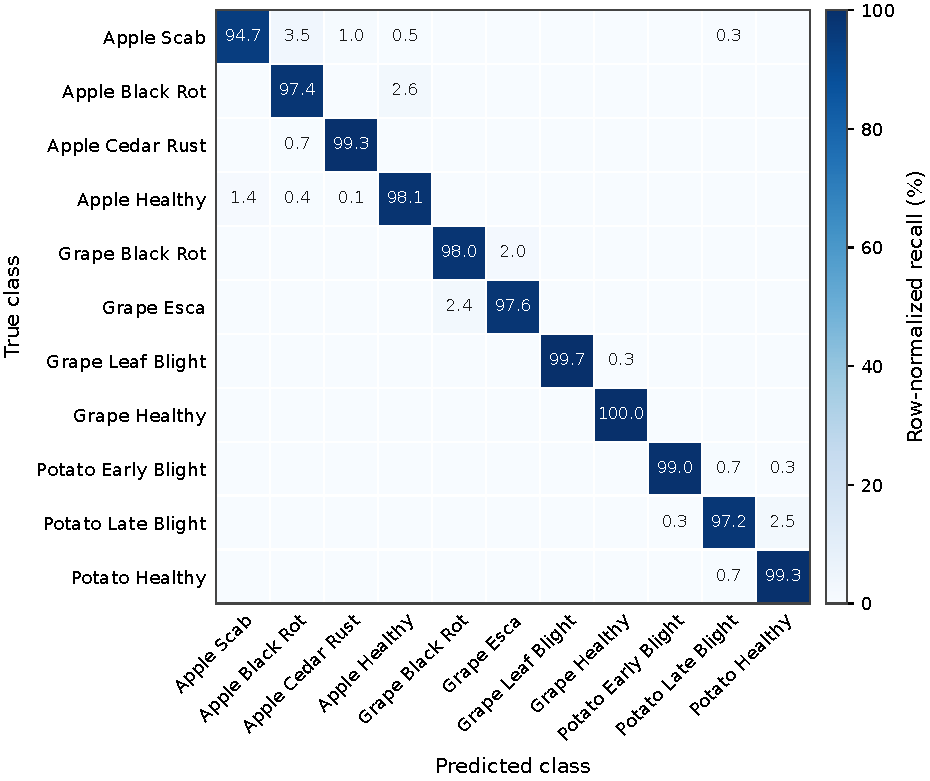
\includegraphics[width=0.82\columnwidth]{fig_confusion.pdf}
\caption{Row-normalized confusion matrix for BioDINO-Edge under transductive inference on the canonical PlantVillage split (9,330 test queries; 11 classes across Apple, Grape, and Potato). Rows represent ground-truth annotations; columns represent predictions. Diagonal entries indicate per-class recall (\%). Residual misclassifications concentrate strictly among pathologies of the same host species; cross-species confusion is negligible (0.021\%).}
\label{fig:confusion}
\end{figure}

\textbf{Diagnostic error patterns and epidemiological containment.} As visualized in Fig.~\ref{fig:confusion}, classification errors are strictly confined within the same botanical host species. Residual confusion occurs primarily between Apple Scab and Apple Black Rot (F1 0.955 and 0.962), where early necrotic spots share visual circularity and chlorotic borders, as well as between intermediate symptom stages of Grape Esca and Grape Black Rot (F1 0.979 and 0.976). Crucially for disease containment, cross-species confusion is near-zero: across 9,330 queries, only two apple scab leaves were misclassified as potato late blight (a 0.021\% error rate). Furthermore, the framework achieves a low false-negative rate of 0.702\% on this canonical split (0.79\% $\pm$ 0.36\% across 30 episodes), misclassifying only 50 out of 7,125 diseased leaves as healthy.
% --- END INLINE: 05_results.tex ---
% --- BEGIN INLINE: 08_discussion.tex ---
% =============================================================================
% 8. PRACTICAL DISCUSSION AND LIMITATIONS
% =============================================================================
\section{Discussion and Practical Limitations}
\label{sec:discussion}

\subsection{Operational Edge Deployment Considerations}
BioDINO-Edge is engineered for operational deployment on resource-constrained agricultural edge platforms, including handheld scouting terminals, tractor-mounted spray booms, and unmanned aerial vehicles (UAVs). By eliminating iterative backpropagation, the framework avoids GPU memory spikes and gradient computation graphs, executing feed-forward inference and closed-form linear algebra directly on ARM CPUs. Under prolonged continuous load, execution throughput settles at 4.26\,FPS (Section~\ref{sec:edge_hardware}); therefore, field deployment is naturally structured around shutter-triggered, on-demand inspections rather than continuous video streams. Furthermore, the modular two-tier architecture enables rapid over-the-air deployment of the lightweight base application ($\approx$22.8\,MB), allowing companion multimodal modules to be downloaded on demand when cellular bandwidth permits. In practical field scouting, agronomists can also dynamically register emerging regional pathogens through the mobile interface using 1--5 symptomatic foliar photos and an optional healthy reference leaf, with closed-form parameter adaptation executing directly on the device CPU.

\subsection{Practical Limitations and Scope}
\textbf{Canopy clutter and leaf segmentation.} BioDINO-Edge processes foliar images at the individual leaf frame level. In unsegmented field imagery with dense, overlapping canopies, multiple leaves from neighboring plants can enter the camera field of view, lowering gating confidence. While tight lesion cropping degrades host context, processing unsegmented canopy clutter introduces irrelevant background vectors. Future work could incorporate leaf segmentation to isolate individual leaves before closed-form classification.

\textbf{Statistical pseudo-replication in support expansion.} Multi-view support expansion generates correlated pseudo-replicates. Because the analytical Ledoit--Wolf shrinkage intensity assumes independent and identically distributed (i.i.d.)\ observations, the nominal $N-C=429$ degrees of freedom overstate the independent information in the support set (effective sample size: 55--440). Although the sensitivity study in Section~\ref{sec:aug_sensitivity} shows that downstream accuracy remains stable across view counts and augmentation modes, a cluster-aware shrinkage estimator that explicitly accounts for within-image dependence remains an important theoretical direction.

\textbf{Attention artifacts in frozen backbones.} Frozen vision transformers can produce high-norm artifact tokens in background regions, and these tokens distort attention maps~\cite{darcet2024vision}. We see similar artifacts on non-symptomatic leaf structures such as veins and petioles. Because Fisher-LDA operates on pooled representations downstream, it does not alter internal backbone attention; the framework targets whole-leaf diagnosis rather than pixel-level lesion localization.

\textbf{Optical degradation and focus blur.} Severe defocus or motion blur degrades fine lesion textures, reducing diagnostic accuracy. The Android client screens frames before diagnosis with two lightweight guards: the maximum cosine similarity between the DINOv2 embedding and the class prototypes must exceed 0.12 for the frame to count as foliage, and the mean luminance of a 64$\times$64 center crop must exceed 22/255 for it to count as illuminated. If either check fails, the application suppresses the diagnosis to prevent false predictions on uninformative frames. An additional discrete-Laplacian variance check (threshold 45) detects motion blur, prompting the user to hold the camera steady when frames are blurred rather than issuing an uncertain diagnosis. While the uncertainty gate routes ambiguous clear foliage to Tier-2, handling optical degradation relies on these front-end guards.

\textbf{Scope and threats to validity.} The physical edge profiling in this work was conducted on a single physical device (Samsung Galaxy S24~FE) with CPU-only INT8 ONNX Runtime; absolute latency and memory will vary across mobile SoCs, though the underlying algorithmic complexity remains hardware-independent. In few-shot evaluation, BioDINO-Edge is designed specifically for streaming, sequential edge inference rather than batch transduction over pre-collected query pools. Finally, while PlantDoc evaluates robustness on unconstrained field foliage with target-domain support, fully unsupervised cross-domain transfer (e.g., PlantVillage$\rightarrow$PlantDoc without target support), quantitative image-quality stress tests, and multi-device profiling remain future research directions.

% =============================================================================
% --- END INLINE: 08_discussion.tex ---
% --- BEGIN INLINE: 09_conclusion.tex ---
% =============================================================================
% 8. CONCLUSION AND FUTURE DIRECTIONS
% =============================================================================
\section{Conclusion and Future Directions}
\label{sec:conclusion}

This paper presented \textbf{BioDINO-Edge}, an on-device few-shot framework for foliar plant disease diagnosis that operates without gradient computation or backpropagation. By coupling frozen vision foundation models (DINOv2 Small) with botanical vision--language encoders (BioCLIP ViT-B/16), the architecture forms a joint 896-dimensional descriptor capturing localized lesion morphology alongside taxonomic context. Regularized Fisher-LDA with Ledoit--Wolf shrinkage resolves the small-sample covariance singularity ($N \ll d$), completing one-time parameter adaptation across all 11 classes in 533.99\,ms on an ARM64 CPU without iterative training. At runtime, per-query diagnosis requires only 59.78\,ms through the Tier-1 fast path, with the dual-metric Shannon-margin uncertainty gate escalating ambiguous foliage to multimodal consensus to achieve an average per-query latency of 149.84\,ms. Across 30 benchmark episodes, BioDINO-Edge achieved 97.41\% $\pm$ 0.71\% accuracy on PlantVillage with a 0.79\% $\pm$ 0.36\% false-negative rate, and reached 84.94\% $\pm$ 11.15\% in 5-way 5-shot field evaluation on PlantDoc (52.38\% across all 27 classes simultaneously), demonstrating efficient, real-time diagnostic capability on commodity edge hardware.

\subsection{Future Directions}
Building upon the operational findings of this work, future research can pursue several directions. First, evaluating and benchmarking the gradient-free pipeline on low-cost embedded single-board computers, such as Raspberry Pi platforms, would support stationary in-field monitoring stations and automated scouting traps. Second, developing blur-robust feature extraction and restoration modules could elevate diagnostic accuracy on optical frames degraded by severe wind-induced canopy motion or camera defocus. Additionally, integrating BioDINO-Edge into the closed-loop controller of an autonomous robotic sprayer for selective, variable-rate nozzle actuation represents a practical pathway toward automated precision crop protection.
% --- END INLINE: 09_conclusion.tex ---
% --- BEGIN INLINE: 10_appendix.tex ---
% =============================================================================
% APPENDIX: REPRODUCIBILITY
% =============================================================================
\appendix
\section{Reproducibility Details}
\label{app:repro}
This appendix specifies the exact splits, seeds, model versions, hyperparameters, and code needed to reproduce every reported number, and states the provenance of each value in Table~\ref{tab:comparative}.

\subsection{Datasets and Splits}
\textbf{PlantVillage (controlled, Table~\ref{tab:comparative}).} We use the 11-class novel subset (Apple, Grape, Potato; 9{,}385 images) with frozen embeddings cached once. Reproducing these controlled runs requires only the cached embeddings and the provided script. \emph{11-class regime:} 30 Monte-Carlo episodes; episode $e$ uses \texttt{random.Random(42+17e)}; for each class the image indices are shuffled, the first 5 form the support and all remaining images form the query (9{,}330 queries/episode; support $\cap$ query $=\emptyset$). \emph{5-way $K$-shot regime:} 50 episodes per $K\in\{1,5,10,15\}$; a single \texttt{random.Random(42)} stream samples 5 of the 11 classes per episode (\texttt{rng.sample(range(11),5)}), shuffles each class, takes the first $K$ as support and the rest as query. All methods share identical support/query indices and cached backbone outputs within each episode. Zero-shot BioCLIP and Tip-Adapter use the BioCLIP branches, whereas centroid and Fisher classifiers evaluate joint BioCLIP+DINOv2 representations to isolate the effect of the adaptation rule.

\textbf{PlantDoc (field domain, labeled target-domain support).} The 27 classes shared by both splits are used; the training-only class (Tomato two-spotted spider mites, 2 images) is dropped, leaving 2{,}668 training and 252 test images. 5-way 5-shot: 50 episodes, \texttt{random.Random(42)}, \texttt{rng.sample(range(27),5)}; 5 support leaves/class drawn from the training split, all test images of the sampled classes as queries. 27-way: 135 support leaves (5/class, 8-view augmented to 1{,}080 feature vectors) and 252 field queries. PlantDoc images come from the original benchmark~\cite{singh2020plantdoc}; the main tables use the 2{,}922-image working redistribution described above, and Appendix~\ref{app:plantdoc_official} compares it with the official release.

\subsection{Full Shot Ladder}
\label{app:shot_ladder}
Table~\ref{tab:shot_ladder} reports diagnostic accuracy across 1-shot, 5-shot, 10-shot, and 15-shot regimes (50 episodes/setting; Appendix~\ref{app:repro}). Zero-shot BioCLIP requires no support labels; minor variation reflects query sampling variance. Published baselines provide literature context under their original protocols (e.g., SC-FSL reports 95\% confidence intervals rather than standard deviations, and class pools differ); studies without verifiable 5-shot metrics (e.g., MAFDE-DN4~\cite{zhao2024mafde}) are discussed qualitatively in Section~\ref{sec:related_work}.

\begin{table*}[htbp]
\caption{Full PlantVillage 5-way shot ladder (accuracy, \%, single-view reference features).}
\label{tab:shot_ladder}
\centering
\footnotesize
\setlength{\tabcolsep}{4pt}
\begin{tabularx}{\textwidth}{@{}X c c c c@{}}
\toprule
\textbf{Method} & \textbf{1-shot} & \textbf{5-shot} & \textbf{10-shot} & \textbf{15-shot} \\
\midrule
\multicolumn{5}{@{}l}{\textit{Controlled evaluations, 11-class pool}} \\
Zero-shot BioCLIP & 38.89$\pm$12.78 & 38.86$\pm$12.79 & 38.83$\pm$12.81 & 38.79$\pm$12.83 \\
Tip-Adapter & 45.15$\pm$13.42 & 68.63$\pm$12.80 & 86.01$\pm$7.49 & 93.23$\pm$4.00 \\
Prototypical Networks & 88.44$\pm$9.13 & 97.45$\pm$2.03 & 98.35$\pm$1.45 & 98.57$\pm$1.27 \\
BioDINO-Edge (inductive) & 88.45$\pm$9.12 & 97.96$\pm$1.85 & 99.10$\pm$0.87 & 99.41$\pm$0.60 \\
BioDINO-Edge (transductive) & 93.42$\pm$6.83 & 98.77$\pm$1.68 & 99.41$\pm$0.60 & 99.63$\pm$0.39 \\
\midrule
\multicolumn{5}{@{}l}{\textit{Published results (context only)}} \\
SC-FSL~\cite{mu2024few} & 78.55$\pm$0.81 & 92.90$\pm$0.47 & -- & -- \\
AgriFewNet~\cite{babu2025agrifewnet} & 87.30 & 94.80 & 97.10 & -- \\
VSF-Trans (Swin-T)~\cite{zhou2026vsf} & 79.01 & 90.51 & -- & -- \\
\bottomrule
\end{tabularx}

\vspace{3pt}
\begin{minipage}{\textwidth}
\footnotesize
\textit{Notes.} Controlled results are mean $\pm$ std over 50 episodes per setting. Published baselines are quoted as reported for context under their original protocols; dashes indicate unreported settings.
\end{minipage}
\end{table*}

\subsection{PlantDoc Release Robustness}
\label{app:plantdoc_official}
The main tables evaluate 2{,}668 training and 252 test images from a 2{,}922-image working redistribution of PlantDoc~\cite{singh2020plantdoc} (omitting two images from the unrepresented spider-mite class). To verify partition robustness, we repeated headline evaluations on the official GitHub release (2{,}342 training / 236 test images) under identical seeds, support sizes, 8-view augmentation, and shrinkage parameters. As reported in Table~\ref{tab:plantdoc_official}, performance differences between the working redistribution and official benchmark release are not statistically significant: 27-way transductive accuracy yields 52.38\% (working) vs.\ 56.78\% (official) ($z=0.98, p=0.33$), and 5-way 5-shot episodic accuracy yields 84.94\% (working) vs.\ 82.17\% (official) (Welch $t=1.15, p=0.25$).

An MD5 (Message Digest Algorithm 5) hash audit identified six test images byte-identical to training samples (four with conflicting annotations in the benchmark). Crucially, none belong to the 135 support leaves ($27 \times 5$), ensuring zero influence on prototype or covariance adaptation. Excluding these six test queries bounds the 27-way accuracy shift to $\pm1.24$\,pp. The partition manifest documenting all 2{,}922 records is published in \path{plantdoc_split_manifest.csv}.

\begin{table}[htbp]
\caption{Headline PlantDoc results on the working redistribution and on the official GitHub release (8-view support expansion).}
\label{tab:plantdoc_official}
\centering
\footnotesize
\setlength{\tabcolsep}{4pt}
\begin{tabular*}{\columnwidth}{@{\extracolsep{\fill}}lcc}
\toprule
\textbf{Regime} & \textbf{Working copy} & \textbf{Official release} \\
 & (2{,}668 / 252) & (2{,}342 / 236) \\
\midrule
27-way inductive & 48.81 & 54.66 \\
27-way transductive & 52.38 & 56.78 \\
27-way macro F1 & 52.52 & 57.33 \\
5-way 5-shot inductive & 82.60$\pm$11.49 & 80.33$\pm$13.94 \\
5-way 5-shot transductive & 84.94$\pm$11.15 & 82.17$\pm$12.86 \\
5-way 5-shot macro F1 & 84.55$\pm$11.20 & 81.48$\pm$13.48 \\
\bottomrule
\end{tabular*}

\vspace{3pt}
\begin{minipage}{\columnwidth}
\footnotesize
\textit{Notes.} Both columns evaluate 8-view support expansion under identical random seeds and shrinkage parameters. Differences between distributions are not statistically significant ($p > 0.25$).
\end{minipage}
\end{table}

\subsection{Models and Hyperparameters}
Table~\ref{tab:hyperparameters} summarizes the architecture specifications, hyperparameter constants, and numerical solver configurations across all evaluation regimes. The Python reference implementation uses \texttt{scikit-learn} with \texttt{solver=lsqr}, while the mobile deployment uses dense Cholesky factorization in EJML. Because conjugate gradients in \texttt{lsqr} solve the identical normal equations, both implementations converge within machine precision. Quantization audits (Table~\ref{tab:quantization}) confirm that end-to-end transductive accuracy changes by at most 0.40\,pp on PlantDoc and 0.24\,pp on PlantVillage under INT8 ONNX execution.

\begin{table}[htbp]
\caption{System hyperparameters and implementation specifications.}
\label{tab:hyperparameters}
\centering
\footnotesize
\setlength{\tabcolsep}{4pt}
\begin{tabularx}{\columnwidth}{@{}l X c@{}}
\toprule
\textbf{Component / Parameter} & \textbf{Symbol / Description} & \textbf{Value / Setting} \\
\midrule
DINOv2 backbone & Frozen visual patch encoder ($d_{\text{dino}}$) & ViT-S/14 (384-D) \\
BioCLIP backbone & Frozen botanical vision--language ($d_{\text{bio}}$) & ViT-B/16 (512-D) \\
Joint representation & Concatenated embedding ($\mathbf{z}$) & 896-D \\
Logit scaling & Cosine temperature ($\gamma$) & 20.0 \\
Fisher blend weight & Inductive blend factor ($w_{\text{lda}}$) & 0.75 \\
Uncertainty gate & Shannon-margin threshold ($\tau$) & 0.35 \\
Transductive support weight & Pseudo-label anchor weighting & $3\times$ \\
Anchor buffer capacity & Maximum anchors per class & 20 \\
Anchor confidence gate & Pseudo-label entry threshold & 0.70 \\
Covariance shrinkage & Regularization estimator & Ledoit--Wolf \\
Singular ridge floor ($N=C$) & Degenerate 1-shot limit & Mean feature variance \\
Tip-Adapter baseline & Blending constants ($\alpha, \beta$) & 1.0, 5.5 \\
Mobile / Server solvers & Dense Cholesky (EJML) $\equiv$ Iterative LSQR & Equivalent ($<10^{-6}$) \\
\bottomrule
\end{tabularx}
\end{table}

\subsection{Environment and Code}
Reference environment: Python 3.12.1, torch 2.6.0 (Compute Unified Device Architecture (CUDA) 12.4 build), scikit-learn 1.9.1, numpy 2.5.4, scipy 1.18.1, timm 1.0.30, open\_clip 3.3.0. Feature extraction ran on an NVIDIA RTX 4070 Laptop GPU, while on-device latency, memory, and thermal profiling executed on the ARM64 CPU of the Galaxy S24 FE. The open-source repository (\url{https://github.com/reyhane-code/BioDINO-Edge}) provides all reproduction scripts and models: (i)~core framework and inference in \path{pipeline/biodino_edge_pipeline.py}; (ii)~ONNX model export and INT8 quantization in \path{pipeline/export_edge_models.py}; (iii)~controlled baselines in \path{experiments/baseline_comparison/run_controlled_baselines.py}; (iv)~canonical PlantVillage validation in \path{experiments/transductive_validation/run_transductive_validation.py}; (v)~routing and gating evaluation in \path{experiments/routing_calibration_validation/run_routing_validation.py}; (vi)~augmentation sensitivity in \path{experiments/augmentation_sensitivity/run_augmentation_sensitivity.py}; and (vii)~mobile profiling reports in \path{experiments/edge_device_benchmark/results/benchmark_report.json}. Edge deployment instructions and pre-quantized models are provided in \path{DEPLOYMENT_GUIDE.md} and \path{models/}.

\subsection{Provenance and Numerical Reproducibility}
Table~\ref{tab:provenance} documents the provenance of reported values (``Re-run'': evaluated locally via reproduction scripts; ``As reported'': transcribed from literature). Controlled reruns reproduce canonical inductive accuracy exactly (95.08\%) and transductive accuracy within 0.04\,pp (97.37\% vs.\ 97.41\% reference, reflecting \texttt{lsqr} solver floating-point sensitivity across library releases, well below the 0.71\,pp standard deviation). Canonical reference values are reported for 11-class benchmarks to ensure consistency with paired significance and sensitivity analyses (Sections~\ref{sec:significance} and~\ref{sec:aug_sensitivity}).

\begin{table}[htbp]
\caption{Provenance of reported values.}
\label{tab:provenance}
\centering

\footnotesize
\begin{tabularx}{\columnwidth}{l X}
\toprule
\textbf{Value} & \textbf{Provenance} \\
\midrule
Table~\ref{tab:comparative} baselines & Re-run, shared splits/seeds; feature branches follow each method \\
Table~\ref{tab:comparative} BioDINO 11-class & Canonical reference run (reproduced $\le$0.04\,pp) \\
Table~\ref{tab:comparative} BioDINO 5-way & Controlled re-run (this work) \\
Table~\ref{tab:shot_ladder} literature rows & As reported, not re-run \\
Table~\ref{tab:plantdoc_context} & Our PlantDoc field-domain run (seeded 8-view ladder, protocol above) \\
Table~\ref{tab:aug_sensitivity} sensitivity & Re-run, this work (same 30-episode protocol) \\
\bottomrule
\end{tabularx}
\end{table}
% --- END INLINE: 10_appendix.tex ---
% --- BEGIN INLINE: 11_backmatter.tex ---
% =============================================================================
% BACK MATTER (ELSEVIER STANDARD FORMAT)
% =============================================================================
\section*{CRediT authorship contribution statement}
\textbf{Reyhane Javidi Alsaadi}: Conceptualization, Methodology, Software, Formal analysis, Investigation, Data curation, Writing - original draft, Visualization.
\textbf{Mohammad Reza Samadzadeh}: Conceptualization, Validation, Writing - review \& editing, Supervision, Project administration.

\section*{Funding}
This research did not receive any specific grant from funding agencies in the public, commercial, or not-for-profit sectors.

\section*{Declaration of Competing Interest}
The authors declare that they have no known competing financial interests or personal relationships that could have appeared to influence the work reported in this paper.

\section*{Data and Code Availability}
The complete open-source mobile application, model export scripts, and evaluation benchmarks are publicly available at \url{https://github.com/reyhane-code/BioDINO-Edge}. The PlantVillage dataset is openly available at \url{https://plantvillage.psu.edu/}, and the PlantDoc benchmark is distributed at \url{https://github.com/pratikkayal/PlantDoc-Dataset}. The main tables use 2{,}668 training and 252 test images from a 2{,}922-image working redistribution; the two training-only tomato two-spotted spider-mite images are excluded. Its split manifest (paths, labels, MD5) is provided as \path{plantdoc_split_manifest.csv}. \ref{app:plantdoc_official} reports the official 2{,}342/236 release.

\section*{Declaration of generative AI and AI-assisted technologies in the writing process}
During the preparation of this work the authors used an AI-assisted tool in order to improve language readability and grammar. After using this tool, the authors reviewed and edited the content as needed and take full responsibility for the content of the published article.

% =============================================================================
% --- END INLINE: 11_backmatter.tex ---

% REFERENCES
% =============================================================================
\bibliographystyle{elsarticle-num}
\bibliography{references}

\end{document}
